\documentclass[11pt]{scrartcl} % Font size

\usepackage{amsmath, amsfonts, amsthm} % Math packages
\usepackage{graphicx} % Required for inserting images
\usepackage[english]{babel}
\setlength\parindent{0pt}
\usepackage{amssymb}
\usepackage{pifont}
\newcommand{\xmark}{\ding{55}}
\usepackage{listings}
\lstset{
  mathescape,         
  literate={->}{$\rightarrow$}{2}
           {ε}{$\varepsilon$}{1}
}

\usepackage{enumitem}

% \def\ContinueLineNumber{\lstset{firstnumber=last}}


% make section font another color
% \usepackage{xcolor}
\usepackage[dvipsnames]{xcolor}
\usepackage{sectsty}
\sectionfont{\color{red}}
\usepackage{wrapfig, booktabs}
\usepackage{algorithm2e}
\SetKwComment{Comment}{\# }{}
\RestyleAlgo{ruled}
\LinesNumbered


%----------------------------------------------------------------------------------------
%	TITLE SECTION
%----------------------------------------------------------------------------------------

\title{	
	\textsc{Knowledge Representation and Reasoning}\\ % Your university, school and/or department name(s)
}

\author{\LARGE Isa-Ali Kirca} % Your name

\date{} % Today's date (\today) or a custom date



\begin{document}

\maketitle % Print the title
\tableofcontents

\newpage

\section{Basics}

\subsection{Symbols}
\begin{tabular}{|l|l|}
\hline
\textbf{\textcolor{red}{Symbol}} & \textbf{\textcolor{red}{Explanation}} \\
\hline
$\neg x$ & negation (not x) \\
\hline
$x \wedge y$ & conjunction (x and y) \\
\hline
$x \vee y$ & disjunction (x or y) \\
\hline
$x \rightarrow y$ \textbf{or} $x \supset y$ & conditional/implies (if x then y) \\
\hline
$x \leftrightarrow y$ \textbf{or} $x \equiv y$ & equivalence/iff (x if and only if y) \\
\hline
$a \models p$ & a satisfies p \\
\hline 
$\forall x$ & for all x \\
\hline
$\exists x$ & there exists x \\
\hline
$\exists !x$ & there is a unique x \\
\hline
\end{tabular}

\vspace{1cm}

\textbf{Truth tables:}
\begin{table}[!htb]
    \begin{minipage}{.1\linewidth}
      \centering
        \begin{tabular}{|l|l|}
            \hline
            \textcolor{red}{x} & $\neg(\text{\textcolor{red}{x}})$ \\
            \hline 
            F & T \\
            \hline
            T & F \\
            \hline
        \end{tabular}
    \end{minipage}%
    \begin{minipage}{.9\linewidth}
      \centering
        \begin{tabular}{| l | l | l | l | l | l |}
            \hline
            \textcolor{red}{x} & \textcolor{red}{y} & $\wedge($\textcolor{red}{x}, \textcolor{red}{y}$)$ & $\vee($\textcolor{red}{x}, \textcolor{red}{y}$)$ & $\rightarrow($\textcolor{red}{x}, \textcolor{red}{y}$)$ & $\leftrightarrow($\textcolor{red}{x}, \textcolor{red}{y}$)$ \\
            \hline
            F & F & F & F & T & T \\
            F & T & F & T & T & F \\
            T & F & F & T & F & F \\
            T & T & T & T & T & T \\
            \hline
        \end{tabular}
    \end{minipage} 
\end{table}

\subsection{Tautology and contradiction}
\begin{table}[!htb]
    \begin{minipage}{.5\linewidth}
      \textbf{\textcolor{red}{Tautology}:} A compound proposition that is always true for all possible truth values of the propositions. \\ \textbf{Example:} $x \vee \neg x$ is a \textcolor{red}{tautology}.
    \end{minipage}
    \begin{minipage}{.5\linewidth}
        \centering
        \begin{tabular}{|l|l|l|}
            \hline
            \textcolor{red}{x} & $\neg($\text{\textcolor{red}{x}}$)$ & \textcolor{red}{x} $\vee$ $\neg$ \textcolor{red}{x} \\
            \hline 
            T & F & T \\
            \hline
            F & T & T \\
            \hline
        \end{tabular}
    \end{minipage}
\end{table}

\begin{table}[!htb]
    \begin{minipage}{.5\linewidth}
      \textbf{\textcolor{PineGreen}{Contradiction}:} A compound proposition that is always false. \\ \textbf{Example:} $x \wedge \neg x$ is a \textcolor{PineGreen}{contradiction}.
    \end{minipage}
    \begin{minipage}{.5\linewidth}
        \centering
        \begin{tabular}{|l|l|l|}
            \hline
            \textcolor{red}{x} & $\neg($\text{\textcolor{red}{x}}$)$ & \textcolor{red}{x} $\wedge$ $\neg$ \textcolor{red}{x} \\
            \hline 
            T & F & F \\
            \hline
            F & T & F \\
            \hline
        \end{tabular}
    \end{minipage}
\end{table}

\begin{table}[!htb]
    \begin{minipage}{.5\linewidth}
      \textbf{\textcolor{NavyBlue}{Contingency}:} A proposition that is \textbf{neither} a \textcolor{red}{tautology} nor \textcolor{PineGreen}{contradiction}.
    \end{minipage}
\end{table}



\newpage
\section{Week 1: Recap IR0}

After gathering the text we want to search, the next step is to decide whether it should be modified or restructured to simplify searching. The types of changes that are made at this stage are called \textbf{text transformation} or, more often, \textbf{text processing}. 
\\
\\
\textbf{\textcolor{Red}{Goal}} of \textbf{text processing}: convert the many forms in which words can occur into more consistent index terms. \\

\begin{tabular}{|l|l|}
\hline
\textbf{Index terms} & representation of the content of a document used for searching. \\
\hline
\textbf{Tokenization}  & words are split apart. Process of forming words from the \\
& sequence of characters in a document. \\
\hline
\textbf{Stopping} & some words may be ignored entirely in order to make \\ & query processing more effective and efficient. \\
\hline
\textbf{Stemming} & allow similar words (like "run" and "running") to match each other. \\
\hline
\end{tabular}
\vspace{0.25cm}

Statistical models of \textbf{word occurrences} are very \textbf{important} in information retrieval, and are used in many of the core components of search engines, such as the ranking algorithms, query transformation, and indexing techniques. One of the most obvious features of text is that the \textbf{distribution of word frequencies} is very \textbf{skewed}. 
\\
\\
\begin{minipage}{.45\textwidth}
\textbf{\textcolor{Maroon}{Zipf's Law}}: the frequency of the $r$th most common word is inversely proportional to $r$ or, alternatively, the rank of a word times its frequency $(f)$ is approx. a constant $(k)$: $r \cdot f = k$.
\\
\\
But we want the probability of occurrence of a word, which is the frequency of the word divided by the total number of word occurrences in the text. In this case, \textcolor{Maroon}{Zipf's law} is: $r \cdot P_r = c$, where $P_r$ is the probability of occurrence for the $r$th ranked word, and $c$ is a constant.
\end{minipage}
\begin{minipage}{.45\textwidth}
  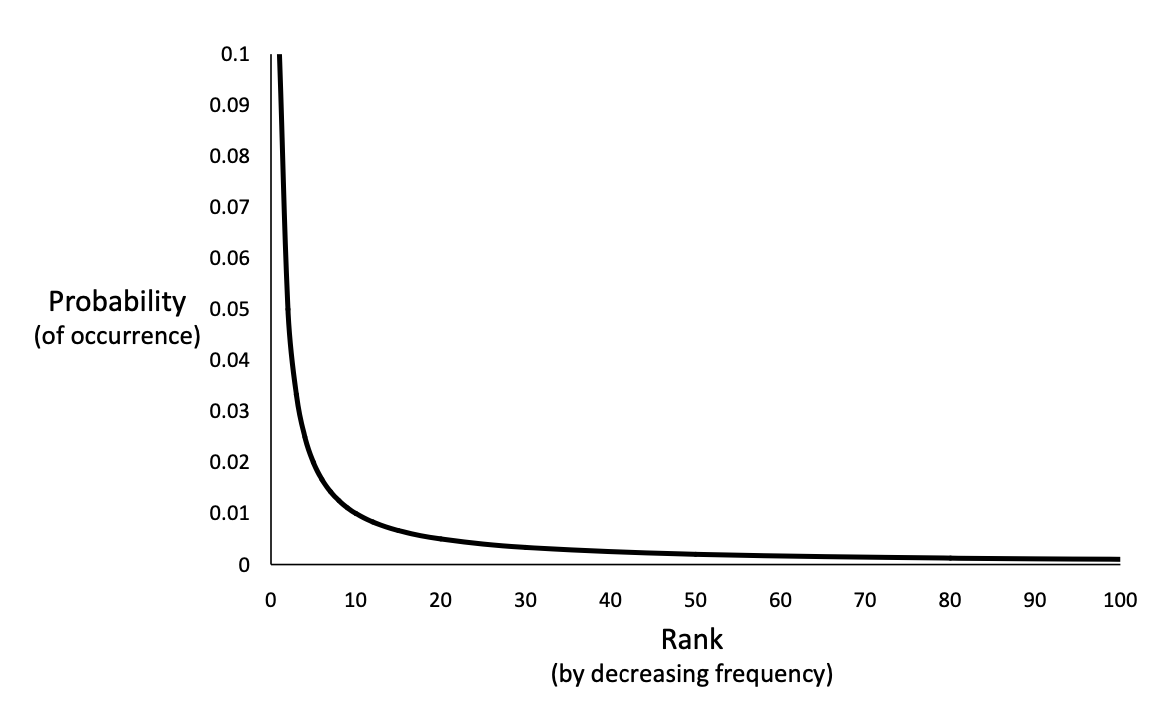
\includegraphics[scale=0.4]{figures/zipf.png}
%   \caption{Tradeoff tools KRR}
\end{minipage}
\vspace{0.35cm}

\textbf{Hapax Legomena}: words that occur once in a text corpus or book.
\\
\\
\textbf{\textcolor{NavyBlue}{Heaps' law}}: Relationship between size of corpus and size of vocabulary.
\\
\\
\begin{minipage}{.3\textwidth}
\centering
$v = k \cdot n^\beta$
\end{minipage}
\begin{minipage}{.7\textwidth}
v = vocabulary size for a corpus of size n words \\
$k$ and $\beta$ = parameters that vary for each collection.
\end{minipage}
\vspace{0.25cm}

\textbf{\textcolor{NavyBlue}{Heaps' law}} predicts that the number of new words will increase very rapidly when the corpus is small and will continue to increase indefinitely, but slower for larger corpora.
\newpage

Word occurrence statistics can also be used to estimate the size of the results from a web search. A \textbf{result} is any document (or web page) that contains all of the query words.  
\\
\\
If we assume that words occur \textbf{\textit{independently}} of each other, then the probability of a document containing all the words in the query is simply the \textbf{product of the probabilities} of the individual words occurring in a document. For example, if there are three query words a, b, and c, then:\\

\begin{minipage}{.4\textwidth}
% \centering
$P(a \cap b \cap c)=P(a) \cdot P(b) \cdot P(c)$
\end{minipage}
\begin{minipage}{.6\textwidth}
% \centering
$P(a \cap b \cap c)$ = \textcolor{Maroon}{joint probability}, or the probability that all three words occur in a document \\
\\
% \centering
$P(a), P(b), P(c)$ =  are the probabilities of each word occurring in a document.
\end{minipage}
\vspace{0.25cm}

A search engine will always have access to the number of documents that a word occurs in $\left(f_{a}, f_{b}\right.$, and $\left.f_{c}\right),$ and the number of documents in the collection $(N)$, so these probabilities can easily be estimated as $P(a)=$ $f_{a} / N, P(b)=f_{b} / N$, and $P(c)=f_{c} / N$:
$$f_{a b c}=N \cdot f_{a} / N \cdot f_{b} / N \cdot f_{c} / N=\left(f_{a} \cdot f_{b} \cdot f_{c}\right) / N^{2} \;\;\;\;\; \text{where $f_{abc}$: estimated size of result set.}$$

\textbf{\textcolor{Maroon}{But}}, this assumption does \textbf{not} lead to good estimates for result size, especially for \textbf{combinations} of \textbf{\textcolor{Maroon}{three words}}. The problem is that the words in these combinations do not occur independently of each other. If we see the word “fish” in a document, for example, then the word “aquarium” is more likely to occur in this document than in one that does not contain “fish”.
\\
\\
Better estimates are possible if \textbf{\textcolor{NavyBlue}{word co-occurrence}} information is also available. Obviously, this would give exact answers for two-word queries. For longer queries, we can improve the estimate by not assuming independence. In general, for three words:
\\

\begin{minipage}{.5\textwidth}
% \centering
$P(a \cap b \cap c)=P(a \cap b) \cdot P(c \mid(a \cap b))$
\end{minipage}
\begin{minipage}{.45\textwidth}
% \centering
$P(a \cap b)$ = probability that the words $a$ and $b$ \textcolor{NavyBlue}{co-occur} in a document \\
\\
$P(a), P(b), P(c)$ =  probability that the word $c$ occurs in a document given that the words $a$ and $b$ occur in the document.
\end{minipage}
\vspace{0.25cm}

These estimates are much better than the ones produced assuming independence, but they are \textbf{still too low}.
\\
\\
Skipped the last few paragraphs of 4.2, because I don't think this is very important.
\newpage

\subsection{Document Parsing}
\textbf{Document parsing} involves recognizing the content and structure of text document.
\\
\\
Metadata is information about a document that is not part of the text content. Metadata content includes document attributes such as date and author, and, most importantly, the \textbf{tags} that are used by \textbf{markup languages} to identify document components. Most popular are HTML and XML.
\\
\\
The \textbf{\textcolor{Red}{parser}} uses the \textbf{tags} and other metadata recognized in the document to interpret the document’s structure based on the syntax of the markup language (\textbf{\textcolor{NavyBlue}{syntactic analysis}}) and to produce a representation of the document that includes both the structure and content. 
\subsection{Tokenizing}
\textbf{\textcolor{Maroon}{Tokenizing}} is the process of forming words from the sequence of characters in a document. Some examples of issues involving tokenizing that can have significant impact on the effectiveness of search are:
\begin{itemize}
    \setlength\itemsep{0em}
    \item \textbf{Small words}: can be important in combination with other words. For example, master, world war II.
    \item \textbf{Hyphenated and non-hyphenated forms of words}
    \item \textbf{Special characters}: important part of the tags, URLs, code, and other important parts of documents that must be correctly tokenized.
    \item \textbf{Capitalized words}: can have different meaning from lowercase words. For ex- ample, “Bush” and “Apple”.
    \item \textbf{Apostrophes}
    \item \textbf{Numbers, including decimals}: for example, nokia 3250, quicktime 6.5 pro.
    \item \textbf{Periods can occur in numbers, abbreviations} (e.g., “I.B.M.”, “Ph.D.”), URLs, ends of sentences, and other situations.
\end{itemize}
\vspace{0.25cm}
Text processing for queries \textbf{\textcolor{Maroon}{must}} be the \textbf{same} as that used for documents. Otherwise, many of the index terms will simply not match the corresponding terms.

\subsection{Stopping}
Human language is filled with function words: words that have little meaning apart from other words. The most popular—“the,” “a,” “an,” “that,” and “those”—are determiners. These words are part of how we describe nouns in text, and express concepts like location or quantity. Prepositions, such as “over,” “under,” “above,” and “below,” represent relative position between two nouns.

In information retrieval, these function words have a second name: \textbf{\textcolor{NavyBlue}{stopwords}}. We call them \textcolor{NavyBlue}{stopwords} because text processing stops when one is seen, and they are thrown out. \textbf{Throwing out} these words \textbf{decreases index size}, \textbf{increases retrieval efficiency}, and generally \textbf{improves retrieval effectiveness}.
\\
\\
Constructing a stopword list must be done with \textbf{\textcolor{Red}{caution}}. Removing too many words will \textbf{\textcolor{Red}{hurt}} retrieval effectiveness.
\\
\\
If storage space requirements allow, it is best to at least index all words in the documents. If stopping is required, the stopwords can always be removed from queries. If keeping stopwords in an index is not possible because of space requirements, as few as possible should be removed in order to maintain maximum flexibility.

\subsection{Stemming}
\textbf{\textcolor{PineGreen}{Stemming}}, also called \textbf{\textcolor{PineGreen}{conflation}}, is a component of text processing that captures the relationships between different variations of a word. More precisely, \textbf{\textcolor{PineGreen}{stemming}} \textbf{reduces} the different forms of a word that occur because of \textbf{\textit{inflection}} (e.g., plurals, tenses) or \textbf{\textit{derivation}} (e.g., making a verb into a noun by adding the suffix -ation) to a common stem.
\\
\\
There are two basic types of \textbf{stemmers}: \textcolor{Maroon}{algorithmic} and \textcolor{NavyBlue}{dictionary}-based. An \textcolor{Maroon}{algorithmic} stemmer uses a small program to decide whether \textbf{two words} are \textbf{related}, usually based on knowledge of word suffixes for a particular language. By contrast, a \textcolor{NavyBlue}{dictionary}-based stemmer has no logic of its own, but instead \textbf{relies} on \textbf{pre-created dictionaries} of related terms to store term relationships.
\\

\begin{minipage}{.5\textwidth}
\textcolor{Maroon}{Algorithmic} stemmers:
\begin{itemize}
    \setlength\itemsep{0em}
    \item \textbf{Suffix-s stemmer}: assumes any word ending in the letter “s” is plural. Cakes $\rightarrow$ cake.
    \item \textbf{Porter stemmer}: consists of a number of steps, each containing a set of rules for removing suffixes. At each step, the rule for the longest applicable suffix is executed. 
\end{itemize}
\end{minipage}
\begin{minipage}{.5\textwidth}
\textcolor{NavyBlue}{Dictionary (Hybrid)}-based stemmers:
\begin{itemize}
    \setlength\itemsep{0em}
    \item \textbf{Krovetz stemmer}: makes constant use of a dictionary to check whether the word is valid. The Krovetz stemmer has the additional advan- tage of producing stems that, in most cases, are full words, whereas the Porter stemmer often produces stems that are word fragments.
\end{itemize}
\end{minipage}
\vspace{0.25cm}

Incorporating language-specific stemming algorithms is one of the most important aspects of customizing, or \textbf{\textcolor{Maroon}{internationalizing}}, a search engine for multiple languages.

\subsection{Phrases and N-grams}
A \textbf{\textcolor{Maroon}{phrase}} is equivalent to a simple \textbf{noun phrase}. This is often restricted even further to include just sequences of nouns, or adjectives followed by nouns. Phrases defined by these criteria can be identified using a \textbf{\textcolor{PineGreen}{part-of-speech (POS) tagger}}. A POS tagger marks the words in a text with labels corresponding to the part-of-speech of the word in that context. Taggers are based on statistical or rule-based approaches and are trained using large corpora that have been manually labeled.
\\
\\
\textbf{\textcolor{Maroon}{N-gram}}: any sequence of $n$ words. \\
\textbf{\textcolor{Maroon}{Unigram}}: single words. \\
\textbf{\textcolor{Maroon}{Bigrams}}: sequences of two words. \\
\textbf{\textcolor{Maroon}{Unigram}}: sequences of three words. \\
\\
The more frequently a word \textbf{\textcolor{Maroon}{N-gram}} occurs, the \textbf{more likely} it is to correspond to a \textbf{meaningful phrase in the language}. N-grams of all lengths form a Zipf distri- bution, with a few common phrases occurring very frequently and a large number occurring with frequency 1. In fact, the rank-frequency data for n-grams (which includes single words) fits the Zipf distribution better than words alone. 

\subsection{Ranking with indexes}
\textcolor{Maroon}{Unsorted arrays} are \textcolor{Maroon}{slow to search}, and \textcolor{RubineRed}{sorted arrays} are \textcolor{RubineRed}{slow at insertion}. By contrast, \textcolor{ForestGreen}{hash tables} and \textcolor{ForestGreen}{trees} are \textcolor{ForestGreen}{fast} for \textcolor{ForestGreen}{both search and insertion}. These structures are more complicated than arrays, but the speed difference is compelling.
\\
\\
\textbf{\textcolor{PineGreen}{Text search}} is very different from traditional computing tasks, so it calls for its own kind of data structure, the \textbf{\textcolor{BlueGreen}{inverted index}}.

\newpage
\subsection{Slides IR0 recap}
\textbf{Outline \textcolor{Maroon}{text analysis}}:
\begin{itemize}
    \setlength\itemsep{0em}
    \item[--] \textbf{Statistical properties of written text} (Zipf's law and Heaps' law)
    \item[--] \textbf{Text analysis pipeline}
    \begin{enumerate}
        \item Remove white-spaces and punctuation
        \item Convert terms to lower-case
        \item Remove stop-words
        \begin{itemize}
            \item[$\circ$] \textcolor{OrangeRed}{Frequency-based}: 
            \begin{itemize}
                \item Set a frequency threshold f
                \item Remove words with the frequency higher than f
            \end{itemize}
            \item[$\circ$] \textcolor{JungleGreen}{Dictionary-based}:
            \begin{itemize}
                \item Create a dictionary of stop-words
                \item Remove words that occur in this dictionary
            \end{itemize}
        \end{itemize}
        \item Convert terms to their stems
        \item Deal with phrases
        \item Apply language-specific processing rules
    \end{enumerate}
    \item[--] \textbf{Stemming}
    \begin{itemize}
        \item[$\circ$] \textcolor{Maroon}{Algorithmic}: Porter-stemmer
        \item[$\circ$] \textcolor{JungleGreen}{Dictionary-based}
        \begin{itemize}
            \item Large dictionary of related words
            \item Semi-automatic: run $\rightarrow$ running, runs, \textcolor{Red}{runned}, \textcolor{Red}{runly}
            \item New-words problem
        \end{itemize}
        \item[$\circ$] \textcolor{DarkOrchid}{Hybrid}: produces words, \textbf{not stems}. Comparable effectiveness with the Porter stemmer
        \begin{itemize}
            \item check the word in a dictionary, \textbf{if found}, leave it as is
            \item if not found, apply algorithmic stemming (remove suffixes)
            \item check the dictionary again
            \item if not found, apply rules to modify the ending
        \end{itemize}
    \end{itemize}
    \item[--] \textbf{Phrases}
    \begin{enumerate}
        \item detect noun phrases using a part-of-speech tagger
        \begin{itemize}
            \item sequences of nouns
            \item adjectives followed by nouns
        \end{itemize}
        \item Detect phrases at the query processing time \\
        Use index with word positions
        \item Use frequent \textbf{n-grams}, e.g., bigrams and trigrams
    \end{enumerate}
\end{itemize}

\newpage
\textbf{Outline \textcolor{Maroon}{indexing}}:
\begin{enumerate}
    \setlength\itemsep{0em}
    \item \textbf{Data structures}: Web Graph, Forward index, Page attribute file, Inverted index
    \item \textbf{Inverted index}
    \begin{enumerate}
        \item Dictionary
        \begin{itemize}
            \item Each entry contains
            \begin{itemize}
                \item Number of pages containing the term
                \item Pointer to the start of the inverted list
                \item Other meta-data about the term
            \end{itemize}
            \item B+ tree, hash table
        \end{itemize}
        \item Inverted lists
        \begin{itemize}
            \item Document identifiers
            \item Frequencies
            \item Positions
            \item Weights
        \end{itemize}
    \end{enumerate}
    \item \textbf{Constructing an index}
    \begin{itemize}
        \item Simple indexer \\
        \textbf{Problems} of this indexer:
        \begin{enumerate}
            \item In-memory:
            \begin{itemize}
                \item Two-pass index
                \item One-pass index with merging
            \end{itemize}
            \item Single-threaded
            \begin{itemize}
                \item Distributed indexing (MapReduce)
            \end{itemize}
        \end{enumerate}
    \end{itemize}
    \item \textbf{Updating an index} \\
    \textbf{Strategies}:
    \begin{itemize}
        \item No merge (low index maintenance cost, high query processing cost)
        \item Incremental update 
        \item Immediate merge (always a single index)
        \item Lazy merge (trade-off between index maintenance and query processing cost)
    \end{itemize}
    \textbf{Page deletions}:
    \begin{itemize}
        \item Maintain identifiers of deleted documents in memory, access during query processing
        \item Garbage collection (e.g., during index merging)
    \end{itemize}
\end{enumerate}
\newpage
\section{Week 2: SAT and DPLL}

\subsection{SAT}
\textbf{The satisfiability problem for propositional logic (SAT)}:
\begin{itemize}
    \item[--] \textbf{Input}: a propositional logic formula $\varphi$ (in CNF)
    \item[--] \textbf{Output}: is there a truth assignment $\alpha$ that satisfies $\varphi$?
\end{itemize}

\textbf{Reminder} solving SAT allows us to perform various reasoning tasks:
\begin{itemize}
    \item[--] $\varphi_1$ \textcolor{PineGreen}{logically entails} $\varphi_2$ ($\varphi_1 \models \varphi_2$) \\ iff $\varphi_1 \wedge \neg \varphi_2$ is \textbf{not satisfiable}.
    \item[--] $\varphi_1$ and $\varphi_2$ are \textcolor{PineGreen}{logically equivalent} ($\varphi_1 \equiv \varphi_2$) \\ iff $(\varphi_1 \wedge \neg \varphi_2) \vee (\varphi_2 \wedge \neg \varphi_1)$ is \textbf{not satisfiable}.
    \item[--] $\varphi$ is \textcolor{PineGreen}{valid} \\ iff $\neg \varphi$ is \textbf{not satisfiable}.
\end{itemize}

\textbf{Algorithms for SAT}:
\begin{itemize}
    \item Most naive algorithm: iterate over all $2^n$ truth assignments\\
    ($n$ is number of propositional variables in formula $\varphi$)
    \item All algorithms for SAT take \textbf{exponential time} in the \textbf{worst case}, but perform \textcolor{PineGreen}{very well} in practice.
    \item Most algorithms work only for \textcolor{blue}{propositional logic} formulas in \textcolor{blue}{CNF}, but translation to CNF often leads to \textbf{\textcolor{red}{exponential blow-up}} in the formula.
\end{itemize}

That's where the \textbf{\textcolor{Maroon}{Tseytin transformation}} comes in handy.

\subsection{Tseytin Transformation}
\begin{itemize}
    \item[--] We can translate an arbitrary propositional logic formula $\varphi$ efficiently to a \\ \textbf{\textcolor{WildStrawberry}{equisatisfiable CNF}} formula $\chi \text{-so } \varphi$ and $\chi$ do not have to be logically equivalent
    \begin{itemize}
        \item[$\circ$] \textbf{\textcolor{WildStrawberry}{Equisatisfiable}}: $\varphi$ is satisfiable iff $\chi$ is satisfiable. 
    \end{itemize}
    \newpage
    \item[--] The \textbf{Tseytin transformation}:
    \begin{itemize}
        \item[$\circ$] Take a formula $\varphi$ and call its variables $p_1, \cdots, p_n$.
        \item[$\circ$] Take all the subformulas $\psi_1, \cdots, \psi_m$ of $\varphi$, where $\psi_1 = \varphi$.
        \item[$\circ$] Introduce new propositional variables $q_1, \cdots, q_m$ -each $q_i$ will represent whether the subformula $\psi_i$ is satisfied.
        \item[$\circ$] For each subformula $\psi_i$, add some clauses to $\chi$:
        \begin{itemize}
            \item If $\psi_i = p_j$, \;\;\;\;\;\;\;\;\;\;\;\;\;\;\; add $(\neg q_i \vee p_j)$ and $(\neg p_j \vee q_i)$; \\
            "$(q_i \leftrightarrow p_j)$"
            \\
            \item If $\psi_i = \neg \psi_j$, \;\;\;\;\;\;\;\;\;\;\;\; add $(\neg q_i \vee \neg q_j)$ and $(q_j \vee q_i)$;  \\ "$(q_i \leftrightarrow \neg q_j)$"
            \\
            \item If $\psi_{i}=\left(\psi_{j} \wedge \psi_{k}\right)$, \;\;\;\; add $\left(\neg q_{i} \vee q_{j}\right),\left(\neg q_{i} \vee q_{k}\right)$, and $\left(\neg q_{j} \vee \neg q_{k} \vee q_{i}\right)$; \\
            $"(q_{i} \leftrightarrow q_{j} \wedge q_{k}))"$
            \\
            \item If $\psi_{i}=\left(\psi_{j} \vee \psi_{k}\right)$, \;\;\;\; add $\left(\neg q_{i} \vee q_{j} \vee q_{k}\right),\left(\neg q_{j} \vee q_{i}\right)$, and $\left(\neg q_{k} \vee q_{i}\right)$; \\
            $"(q_{i} \leftrightarrow (q_{j} \vee q_{k}))"$
            \\
            \item (and similarly for subformulas built using $\rightarrow, \leftrightarrow, ..$)
        \end{itemize} 
        \item[$\circ$] \textbf{Finally}, add the unit clause $(q_1)$.
        \item[$\circ$] Then, $\chi$ is satisfiable iff $\varphi$ is satisfiable. 
    \end{itemize}
\end{itemize}

\subsection{Algorithms}
\subsubsection{Backtracking search}
Main idea of \textbf{\textcolor{PineGreen}{Backtracking search}}:
\begin{itemize}
    \item Pick some truth value for a variable $x$, and try if that leads to a solution. If so, great!
    \item Else (if not), backtrack and try the other value.
\end{itemize}

\textbf{Useful notation}: $\left.\varphi\right|_{\ell}$ ('plugging in' $\ell$ into $\varphi$).
\begin{itemize}
    \item Let $\varphi$ be a CNF formula and $\ell$ a literal;
    \item To obtain $\left.\varphi\right|_{\ell}$ from $\varphi$:
    \begin{enumerate}
        \item Remove all clauses that contain $\ell$ (already satisfied);
        \item Remove $\neg \ell$ from all remaining clauses ($\neg \ell$ cannot be satisfied anymore)
    \end{enumerate}
\end{itemize}

\newpage
\begin{algorithm}
\SetAlgoNoEnd
\SetKwInOut{Input}{Input}
\SetKwInOut{Output}{Output}
\SetKwInput{kwAlgName}{BS$(\varphi, \alpha)$}
\caption{Backtracking search (BS)}\label{alg:BS}
\kwAlgName{}
\Input{a propositional CNF formula $\varphi$, \\ and a partial truth assignment $\alpha$ \textcolor{PineGreen}{\Comment*[r]{$\alpha$ is initially empty}} \vspace{0.1cm}} 
\Output{a satisfying truth assignment $\beta$ for $\varphi$ if it exists, otherwise “unsat” \vspace{0.1cm}}
\Begin{
    \If{$\varphi$ contains the empty clause}{\KwRet{"unsat"} \textcolor{PineGreen}{\Comment*[r]{empty clause means contradiction}}}
    \If{$\varphi$ has no clauses}{\KwRet{$\alpha$} \textcolor{PineGreen}{\Comment*[r]{no clauses means the formula is satisfied}} \vspace{0.25cm}}
    $\ell \gets$ a literal in $\varphi$ not assigned by $\alpha$\ \textcolor{PineGreen}{\Comment*[r]{the branching choice: which $\ell$}}
    \eIf{\textbf{BS}$(\left.\varphi\right|_{\ell}, \alpha \cup\{\ell\} = \beta)$}{\KwRet{$\beta$} \textcolor{PineGreen}{\Comment*[r]{first try $\ell$}}}{\KwRet{\textbf{BS}$(\left.\varphi\right|_{\neg \ell}, \alpha \cup\{\neg \ell\})$} \textcolor{PineGreen}{\Comment*[r]{if $\ell$ did not work, try $\neg \ell$}}}
}
\end{algorithm}

\begin{minipage}[t]{0.2\textwidth}
  \textbf{Ass:} $p_1$
  \centering\raisebox{\dimexpr \topskip-\height}{%
  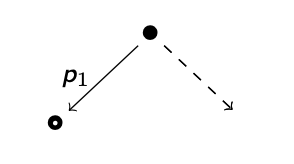
\includegraphics[width=\textwidth]{figures/bs1.png}}
  \label{fig1}
\end{minipage}
\begin{minipage}[t]{0.2\textwidth}
$$
\begin{aligned}
&\left(\text{\textcolor{red}{$\neg p_1$}} \vee \neg p_{2}\right) \\
&\left(\text{\textcolor{red}{$\neg p_1$}} \vee p_{2}\right) \\
\textcolor{Green}{\checkmark} &\left(\text{\textcolor{Green}{$p_1$}} \vee \neg p_{2}\right)
\end{aligned}
$$
\vspace{0.25cm}
\end{minipage}
\begin{minipage}[t]{0.2\textwidth}
  \textbf{Ass:} $p_1 \;\; p_2$
  \centering\raisebox{\dimexpr \topskip-\height}{%
  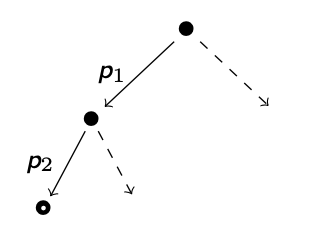
\includegraphics[width=\textwidth]{figures/bs2.png}}
  \label{fig1}
\end{minipage}
\begin{minipage}[t]{0.2\textwidth}
$$
\begin{aligned}
\text{\textcolor{red}{\xmark}} &\left(\text{\textcolor{red}{$\neg p_1$}} \vee \text{\textcolor{red}{$\neg p_{2}$}}\right) \\
\textcolor{Green}{\checkmark} &\left(\text{\textcolor{red}{$\neg p_1$}} \vee \text{\textcolor{Green}{$p_{2}$}}\right) \\
\textcolor{Green}{\checkmark} &\left(\text{\textcolor{Green}{$p_1$}} \vee \text{\textcolor{red}{$\neg p_{2}$}}\right)
\end{aligned}
$$
\end{minipage}

\begin{minipage}[t]{0.2\textwidth}
  \textbf{Ass:} $p_1 \;\; \underline{\text{$\neg p_2$}}$
  \centering\raisebox{\dimexpr \topskip-\height}{%
  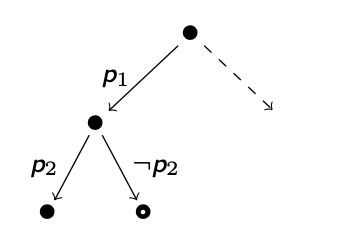
\includegraphics[width=\textwidth]{figures/bs3.png}}
  \label{fig1}
  \vspace{0.25cm}
\end{minipage}
\begin{minipage}[t]{0.2\textwidth}
$$
\begin{aligned}
\text{\textcolor{Green}{\checkmark}} &\left(\text{\textcolor{red}{$\neg p_1$}} \vee \text{\textcolor{Green}{$\neg p_{2}$}}\right) \\
\text{\textcolor{red}{\xmark}} &\left(\text{\textcolor{red}{$\neg p_1$}} \vee \text{\textcolor{red}{$p_{2}$}}\right) \\
\textcolor{Green}{\checkmark} &\left(\text{\textcolor{Green}{$p_1$}} \vee \text{\textcolor{Green}{$\neg p_{2}$}}\right)
\end{aligned}
$$
\end{minipage}
\begin{minipage}[t]{0.2\textwidth}
  \textbf{Ass:} \underline{\text{$p_1$}}
  \centering\raisebox{\dimexpr \topskip-\height}{%
  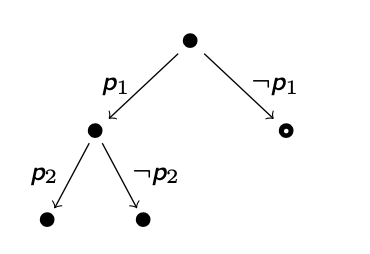
\includegraphics[width=\textwidth]{figures/bs4.png}}
  \label{fig1}
\end{minipage}
\begin{minipage}[t]{0.2\textwidth}
$$
\begin{aligned}
\text{\textcolor{Green}{\checkmark}} &\left(\text{\textcolor{Green}{$\neg p_1$}} \vee \neg p_{2}\right) \\
\textcolor{Green}{\checkmark} &\left(\text{\textcolor{Green}{$\neg p_1$}} \vee p_{2}\right) \\
&\left(\text{\textcolor{red}{$p_1$}} \vee \neg p_{2}\right)
\end{aligned}
$$
\end{minipage}

\begin{minipage}[t]{0.2\textwidth}
  \textbf{Ass:} \underline{\text{$\neg p_1$}} $p_2$
  \centering\raisebox{\dimexpr \topskip-\height}{%
  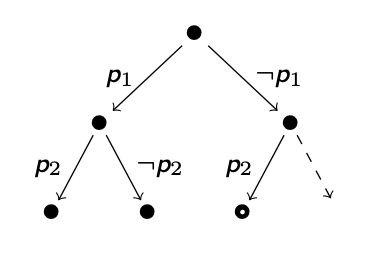
\includegraphics[width=\textwidth]{figures/bs5.png}}
  \label{fig1}
\end{minipage}
\begin{minipage}[t]{0.2\textwidth}
$$
\begin{aligned}
\text{\textcolor{Green}{\checkmark}} &\left(\text{\textcolor{Green}{$\neg p_1$}} \vee \text{\textcolor{red}{$\neg p_{2}$}}\right) \\
\textcolor{Green}{\checkmark} &\left(\text{\textcolor{Green}{$\neg p_1$}}  \vee \text{\textcolor{Green}{$p_{2}$}}\right) \\
\text{\textcolor{red}{\xmark}} &\left(\text{\textcolor{red}{$p_1$}} \vee  \text{\textcolor{red}{$\neg p_{2}$}}\right)
\end{aligned}
$$
\end{minipage}
\begin{minipage}[t]{0.2\textwidth}
  \textbf{Ass:} \underline{\text{$\neg p_1 \neg p_2$}}
  \centering\raisebox{\dimexpr \topskip-\height}{%
  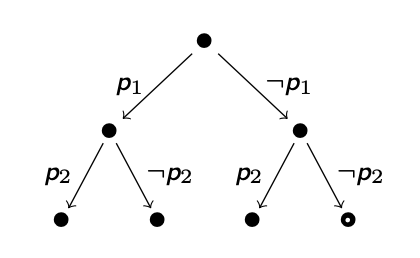
\includegraphics[width=\textwidth]{figures/bs6.png}}
  \label{fig1}
\end{minipage}
\begin{minipage}[t]{0.2\textwidth}
$$
\begin{aligned}
\text{\textcolor{Green}{\checkmark}} &\left(\text{\textcolor{Green}{$\neg p_1$}} \vee \text{\textcolor{Green}{$\neg p_{2}$}}\right) \\
\textcolor{Green}{\checkmark} &\left(\text{\textcolor{Green}{$\neg p_1$}}  \vee \text{\textcolor{red}{$p_{2}$}}\right) \\
\text{\textcolor{Green}{\checkmark}} &\left(\text{\textcolor{red}{$p_1$}} \vee \text{\textcolor{Green}{$\neg p_{2}$}}\right)
\end{aligned}
$$
\vspace{0.1cm}
\end{minipage}

In the example above, we have no empty or no clauses. We start with true, then false and go in ascending order (order picking). Furthermore the dashed line means that we still have to expand this branche later maybe. The colors indicate whether the assignment matches the literal(s). In case the color is \textcolor{red}{red}, the literal is removed from the clause. If all the literals are removed and we have a \textcolor{red}{\xmark}, that branch does not give us a solution, so we need to backtrack to the last point. A \textcolor{Green}{\checkmark} means that the clause is removed. The underlining in the assignment, means that we have no other choice anymore for that literal(s). Once all the clauses have a \textcolor{Green}{\checkmark}, we have a solution.

\newpage
\subsubsection{Propagation: unit propagation (UP)}
\textbf{Propagation}: simplifying the formula at each node in the search tree. \\
\textbf{\textcolor{Maroon}{Unit Propagation}} is a particular propagation method:
\begin{itemize}
    \item If $\varphi$ contains a \textcolor{NavyBlue}{unit clause} ($\ell$), then set the literal $\ell$ to true. 
    \item Repeat this until there are no more unit clauses (or until the formula contains the empty clause)
\end{itemize}
\vspace{0.25cm}
\textbf{\textcolor{WildStrawberry}{DPLL}} makes use of unit propagation.

\begin{algorithm}
\SetAlgoNoEnd
\SetKwInOut{Input}{Input}
\SetKwInOut{Output}{Output}
\SetKwInput{kwAlgName}{DPLL$(\varphi, \alpha)$}
\SetKwInput{kwAlgNameTwo}{UP$(\varphi, \alpha)$}
\caption{DPLL}\label{alg:BS}
\kwAlgName{}
\Input{a propositional CNF formula $\varphi$, \\ and a partial truth assignment $\alpha$ \vspace{0.1cm}} 
\Output{a satisfying truth assignment $\beta$ for $\varphi$ if it exists, otherwise “unsat” \vspace{0.1cm}}
\Begin{
    $(\varphi, \alpha) \gets \text{\textbf{UP}}(\varphi, \alpha)$ \textcolor{PineGreen}{\Comment*[r]{update $(\varphi, \alpha)$ with unit propagation}} 
    \If{$\varphi$ contains the empty clause}{\KwRet{"unsat"}}
    \If{$\varphi$ has no clauses}{\KwRet{$\alpha$} \vspace{0.25cm}}
    $\ell \gets$ a literal in $\varphi$ not assigned by $\alpha$\
    \eIf{\textbf{BS}$(\left.\varphi\right|_{\ell}, \alpha \cup\{\ell\} = \beta)$}{\KwRet{$\beta$}}{\KwRet{\textbf{BS}$(\left.\varphi\right|_{\neg \ell}, \alpha \cup\{\neg \ell\})$}}
}
\vspace{0.5cm}
\kwAlgNameTwo{}
\Begin{
    \While{$\varphi$ contains no empty clause but some unit clause $\ell$
    }{
    $\varphi \gets \left.\varphi\right|_{\ell}$ \textcolor{PineGreen}{\Comment*[r]{$\ell$ must be true, so 'plug in' $\ell$ into $\varphi$}} 
    $\alpha \gets \alpha \cup \left\{ \ell \right\}$ \textcolor{PineGreen}{\Comment*[r]{and add $\ell$ to $\alpha$}}
    }
    \KwRet{ $(\varphi, \alpha)$}
}
\end{algorithm}

The algorithm will still do some things \textcolor{red}{over} and \textcolor{red}{over again}.\\
A way to \textbf{deal} with this: \textbf{\textcolor{NavyBlue}{conflict analysis}} and \textbf{\textcolor{NavyBlue}{clause learning}}.

\newpage
\subsubsection{Conflict graph (implication graph)}

Example of a \textbf{conflict graph}:
\begin{figure}[ht!]
% 	\centering
	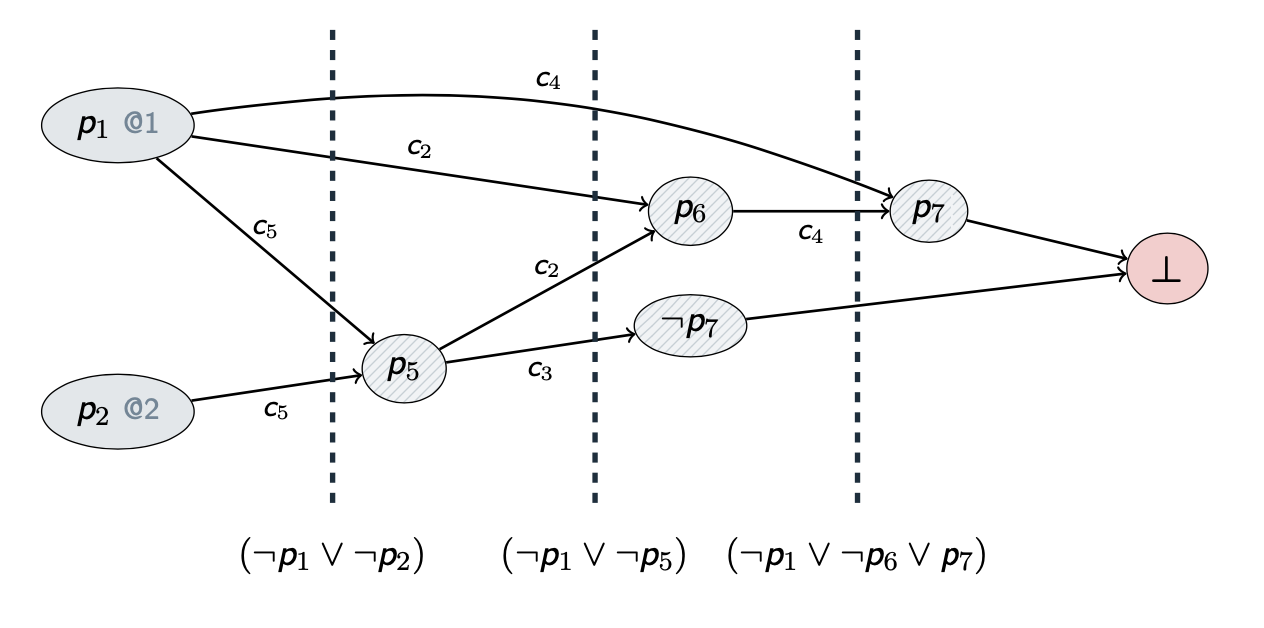
\includegraphics[height=5cm]{figures/conflict graph.png}
	\label{fig:conflict}
\end{figure}

The \textbf{\textcolor{NavyBlue}{implication graph}} is a directed graph that is constructed as follows:
\begin{itemize}
    \item Add a node for each decision literal—i.e., literals that can still be backtracked on.
    \item Every time unit propagation has been used with some clause $(\ell_1 \vee \cdots \vee \ell_k)$ to conclude, say, $\ell_k$ draw an edge from the nodes for $\neg \ell_1, \cdots, \neg \ell_{k-1}$ to the node for $\ell_k$ (and label these edges with the clause number).
    \item Add a node for the conflict (with label $\perp$), and for any two nodes for negated literals (i.e., $\ell$ and $\neg \ell$), draw an edge from these nodes to the conflict node.
\end{itemize}

For each state of the algorithm, there is a unique implication graph—that might contain several pairs of conflicting literals.
\\
\\
A \textbf{\textcolor{Maroon}{conflict graph}} is a subgraph of the \textcolor{NavyBlue}{implication graph} that contains exactly one conflicting pair of literals:
\begin{itemize}
    \item Pick some conflicting pair $\ell, \neg \ell$ of literals in the implication graph, together with the conflict node $\perp$.
    \item Keep only those nodes that have a path to either $\ell$ or $\neg \ell$, and remove all other nodes from the implication graph.
\end{itemize}

\subsubsection{Further additions to DPLL}
\begin{itemize}
    \item \textbf{Pure literal elimination (PL)}: if $\varphi$ contains a literal $\ell$ but not $\neg \ell$, then you can safely set $\ell$ to true.
    \item \textbf{Backjumping}: learning a clause can enable backtracking several choices at once
    \item \textbf{Branching heuristics}: pick a literal $\ell$ that immediately satisfies as many clauses as possible
    \item \textbf{Random restarts}: Restart search every now and then (keep learned clauses).
\end{itemize}

\subsection{SAT and NP-completeness}
A problem Q is \textbf{\textcolor{NavyBlue}{NP-complete}} if every other problem Q' in the class NP can be efficiently (in polynomial-time) be reduced to it (and if Q is in NP).
\begin{itemize}
    \item A \textcolor{red}{reduction} is an algorithm $p$ that maps an input $x^\prime$ for $Q^\prime$ to an input $x$ for $Q$ such that the outputs are the same—e.g., $Q(x) = Q^\prime(x^\prime)$.
\end{itemize}

\textbf{SAT} is \textbf{\textcolor{NavyBlue}{NP-complete}}.

\newpage
\section{Week 3: Logic programming and ASP}

In \textbf{logic programming} you can express \textcolor{Maroon}{facts} and \textcolor{Maroon}{if-then rules}. Example: \textit{Prolog}. \textbf{Goal}: get computationally useful language to represent knowledge and reason with it. \\
\\
\textbf{Positive logic programs} consist of rules and facts (no negations and nots).
\begin{itemize}
    \setlength\itemsep{0em}
    \item \textbf{\textcolor{Maroon}{Rules}} are of the form (can all be true or false):
    \begin{lstlisting}
    a :- b, c, d, ..., z.
    \end{lstlisting}
    \hspace{0.75cm} which represents the implication \textcolor{NavyBlue}{$(b \wedge c \wedge d \wedge \ldots \wedge z) \rightarrow a$}
    \begin{itemize}
        \item \textbf{\textcolor{NavyBlue}{a}} is \textbf{\textcolor{NavyBlue}{head}} of the \textcolor{Maroon}{rule}.
        \item \textbf{\textcolor{NavyBlue}{$b, c, d, \ldots, z$}} is \textbf{\textcolor{NavyBlue}{body}} of the \textcolor{Maroon}{rule}.
    \end{itemize}
    \item \textbf{\textcolor{Maroon}{Facts}} are of the form:
    \begin{lstlisting}
    a.
    \end{lstlisting}
    \hspace{0.75cm} which represents the positive literal \textcolor{NavyBlue}{a}.
\end{itemize}

In \textbf{logic programming}, \textcolor{Maroon}{database semantics} is used:
\begin{itemize}
    \setlength\itemsep{0em}
    \item Objects mentioned are the only objects (\textbf{domain closure})
    \item Objects with different names are different objects (\textbf{unique-names assumption})
    \item (Atomic) statements that are not mentioned are false (\textbf{close-world assumption})
\end{itemize}

So we do not have to explicitly say what \textcolor{Maroon}{function symbols} mean. We can represent \textcolor{Maroon}{objects} simply by the terms that point to them. We can represent the meaning of a \textcolor{Maroon}{relation R} by the set of \textcolor{Maroon}{atoms (over R)} that are true-and then all atoms that are not in this set are false. \\
\\
For \textbf{positive logic programs}, there is a \textbf{\textcolor{Maroon}{unique minimal model}}:
\begin{itemize}
    \item \textcolor{Maroon}{Minimal} in terms of subset-inclusion
    \item \textcolor{Maroon}{Model} is an interpretation that makes all rules true
\end{itemize}

For example the \textcolor{Maroon}{minimal model} for the program below is: $\{a, b, c\}$:
\begin{lstlisting}
a :- b, c.
b :- c.
c.
d :- e.
\end{lstlisting}

We can find this \textbf{\textcolor{Maroon}{minimal model $M$}} with the following procedure:
\begin{enumerate}
    \setlength\itemsep{0em}
    \item Start by putting all facts of the program into $M$.
    \item Repeat until $M$ does not change anymore:\\
    If there is a rule $b \leftarrow c_1,\cdots,c_n$ where $c_1,\cdots,c_n \in M$ put $b$ in $M$ too.
\end{enumerate}

\textbf{Convention to}: write \textcolor{Maroon}{variables} starting with \textcolor{Maroon}{capital letters} and \textcolor{NavyBlue}{relation} and \textcolor{NavyBlue}{function symbols} starting with \textcolor{NavyBlue}{small letters}. \textcolor{Maroon}{Variables} are always \textcolor{Maroon}{universally quantified} ($\forall$).
\newpage

In \textbf{positive logic programs} it is \textbf{not allowed} to use \textcolor{Maroon}{negation} in the \textcolor{Maroon}{body} of rules (\textcolor{Maroon}{not}, which is $\neg$). However, some \textcolor{PineGreen}{extensions} allow this: \textbf{\textcolor{PineGreen}{Datalog}}.\\
\\
In \textbf{\textcolor{PineGreen}{Datalog}}, rules are of the following form:
\begin{lstlisting}
a :- $b_1$, ..., $b_n$, not $c_1$, ..., not $c_m$.
\end{lstlisting}

There are some \textcolor{Maroon}{restrictions} on programs:
\begin{itemize}
    \setlength\itemsep{0em}
    \item Function symbols (with arity $>$ 0) are not allowed
    \item Every variable that appears in the head of a rule, must also appear in a non-negated atom in the body.
    \item Every variable that appears in a negated atom in the body of a rule, must also appear in a non-negated atom in the body.
    \item Negation must be \textcolor{Maroon}{stratified}.
\end{itemize}

\textcolor{Maroon}{Negation} is \textcolor{Maroon}{stratified} in a program P if the following holds:
\begin{itemize}
    \setlength\itemsep{0em}
    \item Draw a directed graph, where the nodes are relation symbols appearing in P.
    \item For every rule $a \text{ :- } b_1, \ldots, b_n, \text{ not } c_1, \ldots, \text{ not } c_m$ in $P$:
    \begin{itemize}
        \item Draw an edge labelled with - (a \textcolor{Maroon}{negative edge}) from the relation symbol in \textcolor{Maroon}{a} to the relation symbol in \textcolor{Maroon}{$c_i$}, for each $1 \leq i \leq m$.
        \item Draw an edge labelled with + (a \textcolor{Maroon}{positive edge})  from the relation symbol in \textcolor{Maroon}{a} to the relation symbol in \textcolor{Maroon}{$b_i$}, for each $1 \leq i \leq n$.
    \end{itemize}
    \item If this graph has no cycles involving negative edges, then negation is \textcolor{Maroon}{stratified}.
\end{itemize}

\begin{figure}[ht!]
	\centering
	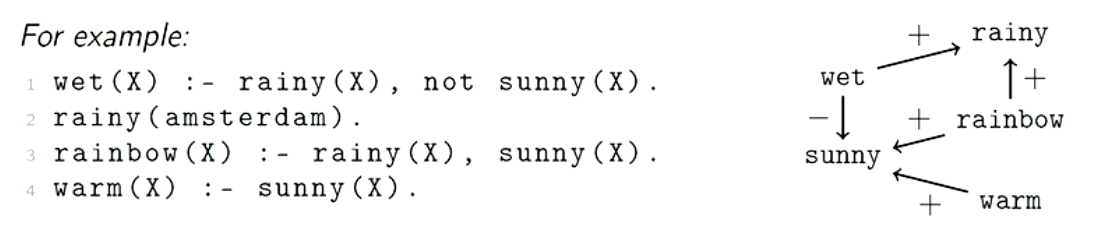
\includegraphics[scale=0.6]{figures/strat.png}
\end{figure}

\textbf{\textcolor{PineGreen}{Datalog}} programs have a \textcolor{Maroon}{unique minimal model} as well.
We can find it with the following procedure:
\begin{enumerate}
    \item Assign a \textcolor{Maroon}{positive integer} to each relation symbol such that: \\
    When there is a negative edge from \textcolor{Maroon}{a} to \textcolor{Maroon}{b}, then the number assigned to \textcolor{Maroon}{a} is strictly largert than that assigned to \textcolor{Maroon}{b} (since there are no cycles with negated edges).
    \item Start by putting all facts of the program into M.
    \item Proceed in stages, one stage for each assigned integer $i$, going from low to high. In each stage $i$:
    \begin{itemize}
        \item Repeat until $M$ does not change anymore: \\
        If there is a rule \textcolor{NavyBlue}{$b \leftarrow c_1, \ldots, c_n \text{ not } d_1, \ldots, \text{ not } d_m$} in $P$ where $c_1, \ldots, c_n \in M$ and $d_1, \ldots, d_m \not \in$, \textcolor{Maroon}{and b is assigned the number $i$}, then put $b$ in $M$ too.
    \end{itemize}
\end{enumerate}

\subsection{Answer Set Programming (ASP)}
What if we want to use negation, but it is not stratified in our knowledge base (\textcolor{Maroon}{unstratified negation})?\\
\\
For example:
\begin{lstlisting}
low :- not high.
high :- not low.
\end{lstlisting}

Then there is \textcolor{Maroon}{not always} a \textcolor{Maroon}{unique minimal model}. In this example, the following are (subset-) minimal models: $\{$low$\}$ and $\{$high$\}$.

\textbf{\textcolor{Maroon}{Answer Set Programming (ASP)}} assigns the so-called \textcolor{Maroon}{answer set semantics} to logic programs with negations. \\
\\
In the basic language of ASP, programs may contain facts and rules of the form:
\begin{lstlisting}
a :- $b_1$, ..., $b_n$, not $c_1$, ..., not $c_m$.
\end{lstlisting}
\begin{itemize}
    \item \textcolor{Maroon}{Negation} does \textcolor{Maroon}{not} have to be \textcolor{Maroon}{stratified}.
    \item It may contain variables, that must appear \textcolor{Maroon}{safely}:
    \begin{itemize}
        \item Every variable that appears in the head of a rule, must also appear in a non-negated atom in the body
        \item Every variable that appears in a negated atom in the body of a rule, must also appear in a non-negated atom in the body.
    \end{itemize}
\end{itemize}

\textbf{Semantics of ASP (intuitions)}:
\begin{enumerate}
    \setlength\itemsep{-0.5em}
    \item Consider an \textcolor{NavyBlue}{interpration M} as \textcolor{Maroon}{an assumption} for which atoms are true and which are false.
    \item Construct a (positive) \textcolor{NavyBlue}{variant $P^M$} of the program $P$ that takes into account this assumption.
    \item Check whether $M$ is the \textcolor{Maroon}{(unique) minimal model of $P^M$}.
\end{enumerate}

\begin{minipage}{0.5\textwidth}
Take a \textcolor{PineGreen}{normal logic program $P$} and an \textcolor{PineGreen}{interpretation $M$}.
\begin{itemize}
    \item The \textcolor{Maroon}{reduct $P^M$} of $P$ w.r.t. $M$ is obtained from $P$ by:
    \begin{enumerate}
        \item removing rules with \textcolor{MidnightBlue}{not a} in the body, for $a \in M$
        \item removing literals \textcolor{MidnightBlue}{not b} from all rules, for $b \not \in M$
    \end{enumerate}
    \item An \textcolor{Maroon}{answer set of $P$} is a set $M$ that is the minimal model of $P^M$.
\end{itemize}
\end{minipage}
\begin{minipage}{0.5\textwidth}
\centering
For example, take \textcolor{MidnightBlue}{$P$} to be: \\
\vspace{0.25cm}
\text{low} :- \text{not high}. \\
\text{high} :- \text{not low}. \\
\vspace{0.25cm}
% \end{lstlisting}
and \textcolor{MidnightBlue}{$M = \{ \text{high} \}$}. Then $P^M$ is: \\
\vspace{0.25cm}
high.\\
\vspace{0.25cm}
and $M$ is the minimal model of $P^M$.
\end{minipage}

\begin{minipage}{0.5\textwidth}
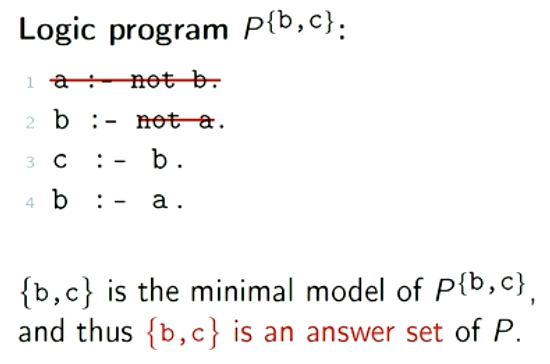
\includegraphics[scale=0.75]{figures/asp1.png}
\end{minipage}
\begin{minipage}{0.5\textwidth}
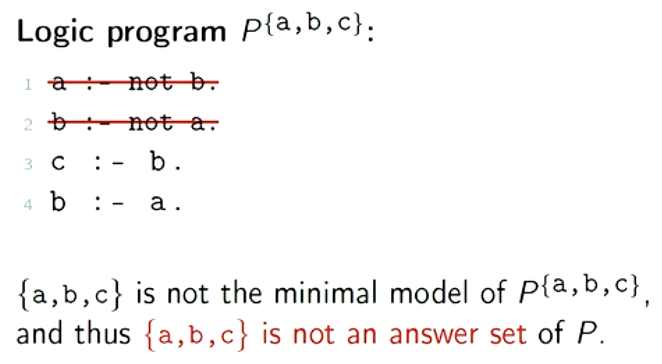
\includegraphics[scale=0.75]{figures/asp2.png}
\end{minipage}

\vspace{0.5cm}

In the figures above:
For any 2 answer sets of a program, they cannot be subsets of each other. The left figure shows that $\{b,c\}$ is an \textcolor{Maroon}{answer set}, which means that $\{a,b,c\}$ cannot be an answer set anymore. \\
\\
Some clarifications:
\begin{itemize}
    \item The first rule in the \textbf{left figure} gets thrown out completely. This is because when building the \textcolor{Maroon}{reduct}, we only look at the literals with \textcolor{Maroon}{not}. So for every \textcolor{Maroon}{not} \textit{something}, where \textit{something} is in the set $P^M$, that rule gets thrown out completely.
    \item In the second rule of the \textbf{left figure} only the right part of the rule gets striked, since we again look at \textcolor{Maroon}{not} \textit{something}, but \textit{something} is not in the set $P^M$. Thus we strike \textbf{not \textit{something}} in that rule.
    \item Thereafter we do the iterative procedure and see that $\{b,c\}$ is the answer set of $P$.
    \item In the \textbf{right figure} we go through the same procedure, except that $\{a,b,c\}$ is not an answer set, since it not the minimal model of $P^{\{a,b,c\}}$
\end{itemize}

\subsection{Building blocks of ASP (- check other PDF)}
\begin{minipage}{0.5\textwidth}
\textbf{Logic program with constraint}:
\begin{lstlisting}
num(1).
num(2).

left(X) :- not right(X), num(X).
right(X) :- not left(X), num(X).

:- left(1), left(2). $\;\;\;\;\;  \text{\textcolor{PineGreen}{\# left(1) and left(2) cannot be true both}}.$
\end{lstlisting}
\end{minipage}
\begin{minipage}{0.5\textwidth}
\textbf{Answer sets (because of constraint)}:
\begin{lstlisting}
num(1) num(2) right(1) left(2)
num(1) num(2) right(1) right(2)
num(1) num(2) left(1) right(2)



.
\end{lstlisting}
\end{minipage}

\vspace{0.25cm}
\textbf{Helpful feature: \# show}: \\
If you want to see a specific part (subset) of the answer set (not changing the problem or answer). 

\newpage
\textbf{Helpful feature: abbreviations}: \\
num(1..3) is equivalent to: num(1). num(2). num(3).  \\
\\
num(a;c) is equivalent to: num(a). num(c). \textbf{So not up to!} \\

\vspace{0.25cm}
\textbf{Helpful feature: \#const}: \\
A constant. So for example \#const k=2 and thereafter num(1, k) will give num(1) up to num(k). \\
\\
\textbf{Choice rules}: \\
Logic program:
\begin{lstlisting}
{ a; b }.
\end{lstlisting}

\begin{minipage}{0.5\textwidth}
Possible translation:
\begin{lstlisting}
a :- not na.
na :- not a.
b :- not nb.
nb :- not b.
\end{lstlisting}
\end{minipage}
\begin{minipage}{0.5\textwidth}
Answer sets:
\begin{lstlisting}
na nb
a nb
na b
a b
\end{lstlisting}
\end{minipage}

\textbf{Choice rule \textcolor{Maroon}{with lower bound}} (choose at least 2 of them): 
\begin{lstlisting}
2 { a; b; c }
\end{lstlisting}
So the anwser set becomes: a b, a c, b c and a b c.\\

\textbf{Choice rule \textcolor{Maroon}{with upper bound}} (choose at most 1 of them): 
\begin{lstlisting}
{ a; b; c } 1
\end{lstlisting}
So the anwser set becomes: \{empty answer set\}, a, and b. \\

\textbf{Choice rule \textcolor{Maroon}{with lower and upper bound}} (choose exactly 2 of them): 
\begin{lstlisting}
2 { a; b; c } 2
\end{lstlisting}
So the anwser set becomes: a b, a c, and b c. \\
\\


{\Large \textbf{\textcolor{Maroon}{Conditional literals (1)}}}: \\
\begin{minipage}{0.6\textwidth}
\textbf{Logic program}:
\begin{lstlisting}
p(1..3).
q(1..2).
s :- p(X) : q(X)
\end{lstlisting}
\end{minipage}
\begin{minipage}{0.3\textwidth}
\textbf{Answer sets}:
\begin{lstlisting}
p(1) p(2) p(3) q(1) q(2) s

.
\end{lstlisting}
\end{minipage}

\newpage

{\Large \textbf{\textcolor{Maroon}{Conditional literals (2)}}}: \\
\begin{minipage}{0.4\textwidth}
\textbf{Logic program}:
\begin{lstlisting}
p(1..3).
q(1..2).
r(1..3).
s :- p(X) : q(X), r(X)
\end{lstlisting}
\end{minipage}
\begin{minipage}{0.6\textwidth}
\textbf{Answer sets}:
\begin{lstlisting}
p(1) p(2) p(3) q(1) q(2) r(1) r(2) r(3) s


.
\end{lstlisting}
\end{minipage}

\vspace{0.35cm}

{\Large \textbf{\textcolor{Maroon}{Conditional literals (3)}}}: \\
\begin{minipage}{0.4\textwidth}
\textbf{Logic program}:
\begin{lstlisting}
p(1..3).
q(1..2).
r(1..3).
t.
s :- p(X) : q(X), r(X) ; t
\end{lstlisting}
\end{minipage}
\begin{minipage}{0.6\textwidth}
\textbf{Answer sets}:
\begin{lstlisting}
p(1) p(2) p(3) q(1) q(2) r(1) r(2) r(3) s t



.
\end{lstlisting}
\end{minipage}

\vspace{0.35cm}

{\Large \textbf{\textcolor{Maroon}{One-to-one mappings}}}: 
\begin{figure}[ht!]
    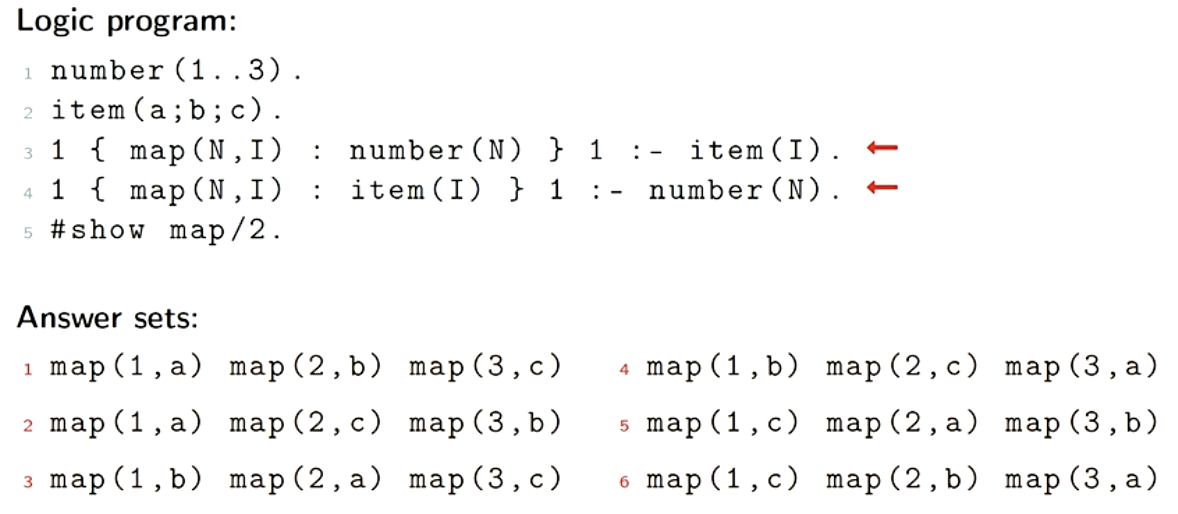
\includegraphics[scale=0.6]{figures/one-to-one.png}
\end{figure}

\newpage
\subsection{Generate and test}
Some useful \textcolor{Maroon}{general guidelines} for modelling a problem in ASP:
\begin{itemize}
    \item Seperate the \textcolor{MidnightBlue}{input} (the encoding of the problem input) from the \textcolor{MidnightBlue}{problem} (the encoding of the solution requirements).
    \item The \textcolor{MidnightBlue}{generate and test} approach.
\end{itemize}

\vspace{0.5cm}

Both have 4 steps:
\begin{enumerate}
    \setlength\itemsep{-0.25em}
    \item \textbf{Formalize the problem}
    \begin{itemize}
        \setlength\itemsep{-0.25em}
        \item What is the \textcolor{Maroon}{problem input}?
        \item What kind of objects are (candidate) solutions?
        \item What properties do solutions need to have?
    \end{itemize}
    \item \textbf{Establish encoding of problem instances}
    \begin{itemize}
        \setlength\itemsep{-0.25em}
        \item What predicates to use to represent the \textcolor{Maroon}{problem input}? What is their arity?
        \item What constants to use to represent the \textcolor{Maroon}{problem input}?
        \item How to translate the \textcolor{Maroon}{problem input} to facts that use these predicates and constants.
    \end{itemize}
    \item \textbf{Establish encoding of candidate solutions (\textcolor{MidnightBlue}{generate})}
    \begin{itemize}
        \setlength\itemsep{-0.25em}
        \item What predicates to use to represent \textcolor{Maroon}{candidate solutions}? What is their arity?
        \item What rules/constraints to add so that the answer sets of the program correspond to all \textcolor{Maroon}{candidate solutions}?
        \item Do you need any auxiliary predicates/rules to express some properties that \textcolor{Maroon}{candidate solutions} should have?
        \item How to obtain from any answer set the corresponding \textcolor{Maroon}{candidate solution}?
    \end{itemize}
    \item \textbf{Establish encoding of solution properties (\textcolor{MidnightBlue}{test})}
    \begin{itemize}
        \setlength\itemsep{-0.25em}
        \item What rules/constraints to add so that only the answer sets remain that correspond to \textcolor{Maroon}{actual solution}?
        \item Do you need any auxiliary predicates/rules to express some properties that \textcolor{Maroon}{actual solutions} should have?
    \end{itemize}
\end{enumerate}

\newpage
\textbf{Example:} 
\begin{figure}[ht!]
    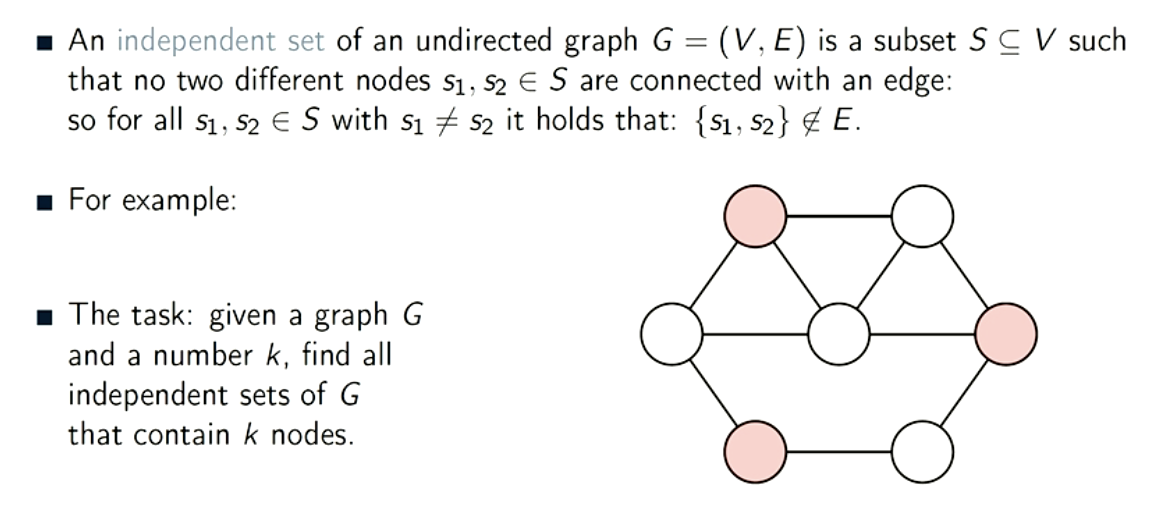
\includegraphics[scale=0.6]{figures/example 1.png}
\end{figure}


\begin{minipage}{0.5\textwidth}
    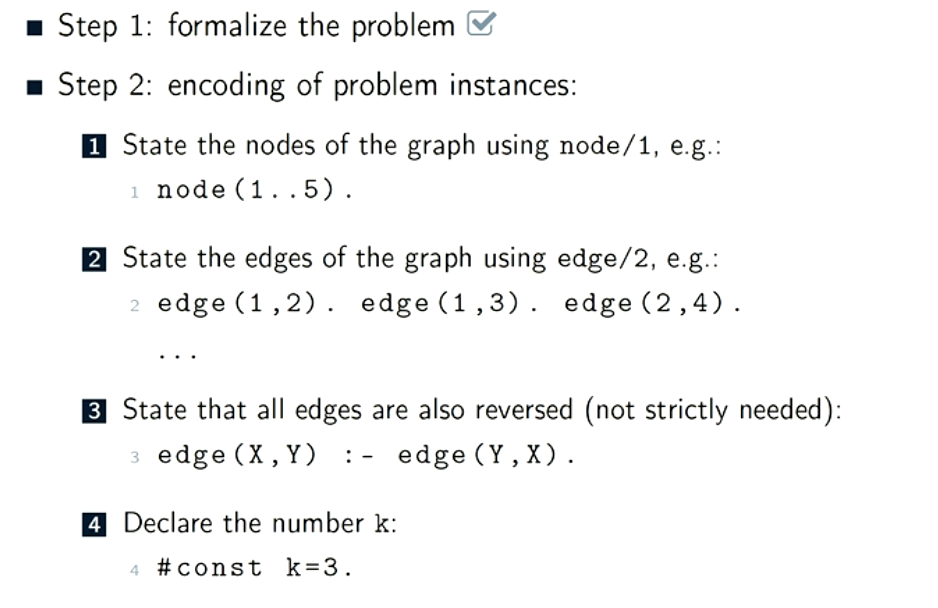
\includegraphics[scale=0.5]{figures/example 2.png}
\end{minipage}
\begin{minipage}{0.5\textwidth}
    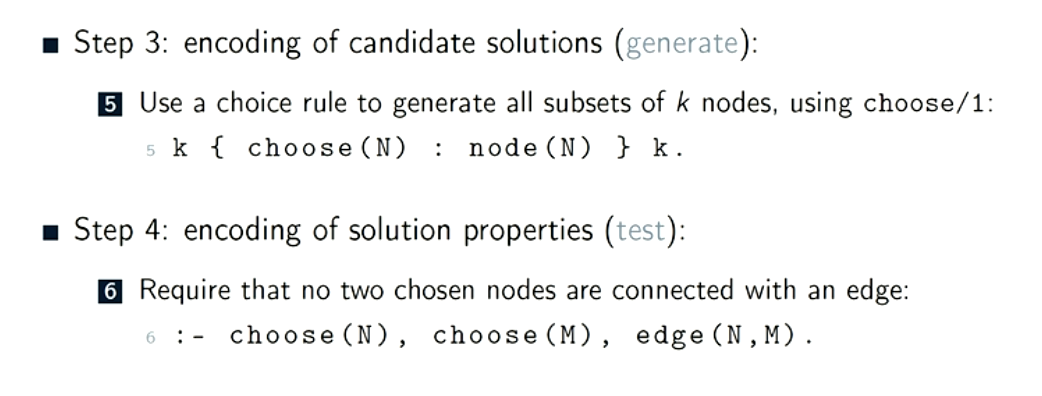
\includegraphics[scale=0.5]{figures/example 3.png}
\end{minipage}

\subsection{Grounding}
{\Large \textbf{\textcolor{Maroon}{Grounding algorithm}}}:
\begin{itemize}
    \setlength\itemsep{-0.25em}
    \item Keep track of a set $D$ of atoms that appear in the head of some ground rule. Initially, $D$ contains the facts of the program $P$.
    \item Apply the following procedure, until $D$ does not change anymore:
    \begin{itemize}
        \setlength\itemsep{-0.25em}
        \item If there is a ground version of some rule in $P$ where all non-negated atoms in the body appear in $D$, add the head of the rule to $D$.
    \end{itemize}
    \item For example:
    \begin{lstlisting}
    path(a,b).
    path(b,c).
    path(X,Z) :- path(X, Y), path(Y,Z).
    \end{lstlisting}
    \begin{itemize}
        \setlength\itemsep{-0.25em}
        \item initially, \textcolor{MidnightBlue}{$D = \{\text{ path}(a,b). \text{ path}(b,c) \; \}$}
        \item One instantiation with atoms in $D$: \textcolor{MidnightBlue}{$\text{path}(a,c) \text{ :- } \text{path}(a,b), \text{ path}(b,c).$}
        \item Then, \textcolor{MidnightBlue}{$D = \{ \text{ path}(a,b). \text{ path}(b,c). \text{ path}(a,c) \;  \}$}, and the algorithm stops.
    \end{itemize}
\end{itemize}

\newpage
{\Large \textbf{\textcolor{Maroon}{Safety}}}: \\
To carry out this 'on demand' grounding, all rules and constraints need to have a property of \textcolor{Maroon}{safety}:
\begin{itemize}
    \item A rule/constraint is called \textcolor{Maroon}{safe} if every variable appearing in it appears at least once in the body in an unnegated literal.
\end{itemize}

\textbf{Examples}:  \\
Safe:
\begin{lstlisting}
a(X,Y,Z) :- b(X,Y), c(X,Z), not d(X,Y,Z)
\end{lstlisting}

Not safe:
\begin{lstlisting}
a(X,Y,Z) :- b(X,Y) not d(X,Y,Z)
\end{lstlisting}

Not safe (be careful with negated statements):
\begin{lstlisting}
a(X,Y,Z) :- b(X,Y), X + Y != Z $\textcolor{PineGreen}{\text{\;\;\;\; \# Z is unsafe here}}$
\end{lstlisting}
\section{Week 4: Learning to Rank (LTR) and Interactions}

\subsection{Preliminaries and Goal} 

\textbf{Representation}: \\
Represent the document and query in a format that a ML model can use: \textcolor{Maroon}{a numerical vector} $\vec{x} \in \mathbb{R}^{n}$.\\
\\
\textbf{Prediction}: \\
Then a \textcolor{Maroon}{ranking model} $f : \vec{x} \rightarrow \mathbb{R}$ is optimized to score each document-query combination so that relevant documents are scored higher. \\
In mathematical terms: $f$ maps a vector to a real-valued score. \\
\\
\textbf{Features}: \\
Traditionally features are hand-crafted to encode IR insights, nowadays we also have \textit{\textcolor{MidnightBlue}{deep learned}} features. \\
\\
They can be categorized as: 
\begin{itemize}
    \setlength\itemsep{0em}
    \item \textbf{\textcolor{Maroon}{Document-only}} or static features (e.g., document length)
    \item \textbf{\textcolor{Maroon}{Document-Query-combination}} or dynamic features (e.g., BM25)
    \item \textbf{\textcolor{Maroon}{Query-only}} features (e.g., query length)
\end{itemize}

\newpage
\textbf{Models can be trained on different data}:
\begin{itemize}
    \setlength\itemsep{0em}
    \item \textbf{\textcolor{Maroon}{Offline or Supervised}} LTR: learn from annotated data.
    \begin{itemize}
    \setlength\itemsep{0em}
        \item Expensive and time consuming.
        \item Provides ground truth
    \end{itemize}
    \item \textbf{\textcolor{Maroon}{Online/Counterfactual}} LTR: learn from user interactions.
    \begin{itemize}
    \setlength\itemsep{0em}
        \item Virtually free and easy to obtain.
        Hard to interpret.
    \end{itemize}
\end{itemize}

\subsection{Offline LTR}
Data is obtained by:
\begin{enumerate}
\setlength\itemsep{0em}
    \item Pay some humans to be annotators (and train them to be good annotators).
    \item Collect a set of queries
    \item Preselect a large (not too large) set of documents per query.
    \item Show document-query pairs to annotators.
    \item Annotators rate every document-query pair on their relevance (e.g. on a scale from 0 to 4).
\end{enumerate}

\textbf{Goal}: \\
We have:
\begin{itemize}
\setlength\itemsep{0em}
    \item Feature representation of document-query pairs: $\vec{x}_{q,d} \in \mathbb{R}$.
    \item Labels indicating the relevance of document-query pairs: $y_{q,d} \in [0,4]$
\end{itemize}

And we want:
\begin{itemize}
\setlength\itemsep{0em}
    \item A function $f: \vec{x} \rightarrow \mathbb{R}$ that scores documents.
    \item To get the best ranking by sorting according to $f(\vec{x})$.
\end{itemize}

How to find $f$?

\subsection{Pointwise approach}
Regression-based or classification-based approaches are popular. \\
\\
\textbf{Regression loss}: \\
Given $\langle q, d\rangle$ predict the value of $y_{q,d}$. \\
\\
E.g., \textcolor{MidnightBlue}{square loss} for binary or categorical labels:
$$ \mathcal{L}_{\text {Squared }}\left(q, d, y_{q, d}\right)=\left\|y_{q, d}-f\left(\vec{x}_{q, d}\right)\right\|^{2} $$

where $y_{q,d}$ is the one-hot representation or the actual value of the label.

\textbf{Classification loss}: \\
Given $\langle q, d\rangle$ predict the class $y_{q,d}$. \\
\\
E.g., \textcolor{MidnightBlue}{Cross-Entropy} with \textcolor{MidnightBlue}{Softmax} over categorical labels $Y$:
$$ \mathcal{L}_{\mathrm{CE}}\left(q, d, y_{q, d}\right)=-\log \left(p\left(y_{q, d} \mid q, d\right)\right)=-\log \left(\frac{e^{\sigma \cdot s_{y_{q, d}}}}{\sum_{y \in Y} e^{\sigma \cdot s_{y}}}\right) $$

where $s_{y_{q, d}}$ is the model's score for label $y_{q,d}$.\\
\\
\textbf{\textcolor{Red}{Issues}} with \textbf{pointwise approaches}:
\begin{itemize}
\setlength\itemsep{0em}
    \item \textbf{Class imbalance}: many irrelevant documents and very few relevant documents.
    \item \textbf{Query level feature normalization needed}: distr. of features differs greatly per query
\end{itemize}

\textcolor{Maroon}{But}, these can be overcome. \\
\\

\textbf{The \textcolor{Red}{fundamentally wrong part} is}: \\
\textcolor{Maroon}{Ranking is not a regression or classification problem}. \\
\\
A document-level loss does not work for raking problems because document scores should not be considered independently (\textcolor{Maroon}{pointwise methods do not directly optimize ranking quality}). 
\subsection{Pairwise approach}
Instead of looking at document-level, consider \textcolor{MidnightBlue}{pairs of documents}. 
$$ P\left(d_{i} \succ d_{j}\right)=f\left(\vec{x}_{i}, \vec{x}_{j}\right) $$

Do \textcolor{Maroon}{not} change the model to take \textcolor{Maroon}{document pairs as input} (would be quadratic in complexity: $O\left(N^{2}\right)$, during \textcolor{Maroon}{inference}). \\
\\
The scoring model remains \textcolor{Maroon}{unchanged}: $f(\vec{x_i}) = s_i$, but the \textcolor{MidnightBlue}{loss function} is based on \textcolor{Maroon}{document pairs}:
$$ \mathcal{L}_{\text {pairwise }}=\sum_{d_{i} \succ d_{j}} \phi\left(s_{i}-s_{j}\right) $$

Thus we still score documents and then order according to scores.
\newpage
\textbf{\textcolor{Red}{Pairwise loss functions}}: \\
Pairwise loss minimizes the \textcolor{Maroon}{average number of inversions} in ranking: \\
$d_{i} \succ_{q} d_{j}$ but $d_{j}$ is ranked higher than $d_{i}$\\
\\
\textbf{Generally} the following form: 
\begin{equation*}
    \mathcal{L}_{\text {pairwise }}=\phi\left(s_{i}-s_{j}\right)
\end{equation*}

where $\phi$ can be:
\begin{itemize}
\setlength\itemsep{0em}
    \item \textbf{Hinge function}: $\phi(z) = \max(0, 1-z)$
    \item \textbf{Exponential function}: $\phi(z) = e^{-z}$
    \item \textbf{Logistic function}: $\phi(z) = \log(1 + e^{-z}$
    \item etc.
\end{itemize}
\vspace{0.5cm}
{\Large \textbf{\textcolor{NavyBlue}{RankNet}}} (using $\sigma$ instead of $\gamma$, following assignment notation): \\
is a pairwise loss function - popular choice for training neural LTR models. \\
\\
For a given query, each pair of documents $D_{i}$ and $D_{j}$ with differing labels is chosen, and each such pair (with feature vectors $x_{i}$ and $x_{j}$) is presented to the model, which computes the scores $s_{i}=f\left(x_{i}\right)$ and $s_{j}=f\left(x_{j}\right)$. Let $D_{i} \triangleright D_{j}$ denote the event that $D_{i}$ should be ranked higher than $D_{j}$. The two outputs of the model are mapped to a learned probability that $D_{i}$ should be ranked higher than $D_{j}$ via a sigmoid function:\\
\\
\begin{minipage}{0.6\textwidth}
\textcolor{Maroon}{Predicted probabilities}:
\begin{align*}
    &P_{ij} = P(D_{i} \triangleright D_{j}) \equiv \frac{1}{1+e^{-\sigma\left(s_{i}-s_{j}\right)}} \\
    &P_{ji} = P(D_{i} \triangleleft D_{j}) \equiv \frac{1}{1+e^{-\sigma\left(s_{j}-s_{i}\right)}}
\end{align*}
\end{minipage}
\begin{minipage}{0.4\textwidth}
\textcolor{Maroon}{Desired probabilities}:
\begin{align*}
    \bar{P}_{i j}=1 \\
    \bar{P}_{ji}=0
    \\
\end{align*}
\end{minipage}

\vspace{0.5cm}

Computing \textbf{cross-entropy} between $\bar{P}$ and $P$:
\begin{equation*}
\begin{aligned}
\mathcal{L}_{\text {RankNet }} &=-\bar{P}_{i j} \log \left(P_{i j}\right)-\bar{P}_{j i} \log \left(P_{j i}\right) \\
&=-\log \left(P_{i j}\right) \\
&=\log \left(1+e^{-\sigma\left(s_{i}-s_{j}\right)}\right)
\end{aligned}
\end{equation*}

\textbf{\textcolor{Maroon}{Factorization}} \textcolor{NavyBlue}{RankNet}: let $S_{ij} \in \{-1, 0, 1\}$ indicate the preference between $d_i$ and $d_j$. \\
\\
\begin{minipage}{0.5\textwidth}
\textcolor{Maroon}{Predicted probabilities}:
\begin{align*}
    \bar{P}\left(d_{i} \succ d_{j}\right)=\frac{1}{2}\left(1+S_{i j}\right)
\end{align*}
\end{minipage}
\begin{minipage}{0.5\textwidth}
\textcolor{Maroon}{Desired probabilities}:
\begin{align*}
    P\left(d_{i} \succ d_{j}\right)=\frac{1}{1+e^{-\sigma\left(s_{i}-s_{j}\right)}}
\end{align*}
\end{minipage}

\vspace{0.25cm}

\textbf{The cross-entropy loss} is then:
\begin{align*}
    \mathcal{L}_{i j}=\frac{1}{2}\left(1-S_{i j}\right) \sigma\left(s_{i}-s_{j}\right)+\log \left(1+e^{-\sigma\left(s_{i}-s_{j}\right)}\right)
\end{align*}

\newpage

We can also consider a \textbf{\textcolor{Maroon}{sped-up version}} of the \textcolor{NavyBlue}{RankNet}: \\
First we need the derivative w.r.t. $s_i$: 
\begin{align*}
    \frac{\delta \mathcal{L}_{i j}}{\delta s_{i}}=\sigma\left(\frac{1}{2}\left(1-S_{i j}\right)-\frac{1}{1+e^{-\sigma\left(s_{i}-s_{j}\right)}}\right)=-\frac{\delta \mathcal{L}_{i j}}{\delta s_{j}}
\end{align*}

We can further factorize this loss so that:
\begin{align*}
    \frac{\delta \mathcal{L}_{i j}}{\delta w}=\frac{\delta \mathcal{L}_{i j}}{\delta s_{i}} \frac{\delta s_{i}}{\delta w}+\frac{\delta \mathcal{L}_{i j}}{\delta s_{j}} \frac{\delta s_{j}}{\delta w}=\sigma\left(\frac{1}{2}\left(1-S_{i j}\right)-\frac{1}{1+e^{-\sigma\left(s_{i}-s_{j}\right)}}\right)\left(\frac{\delta s_{i}}{\delta w}-\frac{\delta s_{j}}{\delta w}\right)
\end{align*}

\vspace{0.25cm}

The factorized \textbf{cross entropy loss}:
\begin{align*}
    \frac{\delta \mathcal{L}_{i j}}{\delta w}=\sigma\left(\frac{1}{2}\left(1-S_{i j}\right)-\frac{1}{1+e^{-\sigma\left(s_{i}-s_{j}\right)}}\right)\left(\frac{\delta s_{i}}{\delta w}-\frac{\delta s_{j}}{\delta w}\right)
\end{align*}

We choose $\lambda$ so that:
\begin{align*}
    \frac{\delta \mathcal{L}_{i j}}{\delta w}=\lambda_{i j}\left(\frac{\delta s_{i}}{\delta w}-\frac{\delta s_{j}}{\delta w}\right)
\end{align*}

where:
\begin{align*}
    \lambda_{i j}=\sigma\left(\frac{1}{2}\left(1-S_{i j}\right)-\frac{1}{1+e^{-\sigma\left(s_{i}-s_{j}\right)}}\right)
\end{align*}

These \textcolor{Maroon}{lambdas} act like \textbf{forces} pushing pairs of documents apart or together. \\
\\
\textcolor{Maroon}{On document level the same can be done (will copy-paste directly from the paper, since the slides didn't help me)}:
\\
\\
Let $I$ denote the set of pairs of indices $\{i, j\}$, for which we desire $D_{i}$ to be ranked differently from $D_{j}$ (for a given query). $I$ must include each pair just once, so it is convenient to adopt the convention that $I$ contains pairs of indices $\{i, j\}$ for which $D_{i} \triangleright D_{j}$, so that $S_{i j}=1$ (which simplifies the notation considerably, and we will assume this from now on). Note that since RankNet learns from probabilities and outputs probabilities, it does not require that the documents are labeled; it just needs the set $I$, which could also be determined by gathering pairwise preferences. \\
\\
Now we introduce the $\lambda_{i}$ (one $\lambda_{i}$ for each document: note that the $\lambda$ 's with one subscript are sums of the $\lambda$ 's with two). To compute $\lambda_{i}$ (for document $D_{i}$ ), we find all $j$ for which $\{i, j\} \in I$ and all $k$ for which $\{k, i\} \in I$. For the former, we increment $\lambda_{i}$ by $\lambda_{i j}$, and for the latter, we decrement $\lambda_{i}$ by $\lambda_{k i}$. For example, if there were just one pair with $D_{1} \triangleright D_{2}$, then $I=\{\{1,2\}\}$, and $\lambda_{1}=\lambda_{12}=-\lambda_{2}$. In general, we have:
$$
\lambda_{i}=\sum_{j:\{i, j\} \in I} \lambda_{i j}-\sum_{j:\{j, i\} \in I} \lambda_{i j}
$$

\newpage
\textbf{\textcolor{Red}{Issues}} with \textbf{pointwise approaches}:
\begin{itemize}
\setlength\itemsep{0em}
    \item \textbf{RankNet based on virtual probabilities}: $P\left(d_{i} \succ d_{j}\right)$ \\
    In reality the ranking model does not follow these probabilites. 
\end{itemize}

\textcolor{Maroon}{But}, not a big deal. \\

\textbf{The \textcolor{Red}{fundamentally wrong part} is}: \\
Not \textcolor{Maroon}{every document pair} is \textcolor{Maroon}{equally important}.
\\
\\
\textbf{It is \textcolor{Maroon}{Much more important} to get the \textcolor{Maroon}{correct ordering of top documents} than of
the bottom documents} (top 5 more important than order of documents after position 10).

\subsection{Listwise approach}
The \textbf{\textcolor{Maroon}{fundamental problem}} with the approaches so far is that they did \textbf{\textcolor{Maroon}{not optimize ranking quality} directly}.

A \textbf{LTR method} should \textbf{directly optimize the ranking metric} we care about (from simple to more complex):
\begin{itemize}
\setlength\itemsep{0em}
    \item Simple: \\
    $$ \text{precision}(R) = \frac{1}{|R|} \sum_{R_{i}} \text { relevance }\left(R_{i}\right) $$
    \item Complex (e.g., discounted cumulative gain): \\
    $$
D C G(R)=\sum_{R_{i}} \frac{2^{\operatorname{relevance}\left(R_{i}\right)}-1}{\log (i+1)}
$$
\end{itemize}

\textbf{These metrics are \textcolor{Maroon}{non-continuous} and \textcolor{Maroon}{non-differentiable}}. \\
\\
Due to \textcolor{Maroon}{strong position-based discounting in IR measures}, \textbf{errors at higher ranks} are \textcolor{Maroon}{much more problematic} than at lower ranks. \\
\\
{\Large \textbf{\textcolor{NavyBlue}{LambdaRank}}}: \\
Multiply actual gradients with the change in NDCG by swapping the rank positions of the two documents:
$$ \lambda_{L a m b d a R a n k}=\lambda_{R a n k N e t} \cdot|\Delta \mathrm{NDCG}| $$

Works also with other metrics, e.g. $\mid \Delta$ Precision $\mid $.\\
\\
\textbf{Empirically, \textcolor{MidnightBlue}{LambdaRank} was shown to \textcolor{Maroon}{directly optimize IR metrics}}. Theoretically was shown, that \textcolor{MidnightBlue}{LambdaRank} \textcolor{Maroon}{optimizes a lower bound} on certain IR metrics.

\newpage

\subsection{ListNet and ListMLE}
Create a probabilistic model for ranking, which is differentiable. \\
\\
\begin{minipage}{0.6\textwidth}
Sample documents from a \\ \textcolor{Maroon}{Plackett-Luce distribution}:
$$ P\left(d_{i}\right)=\frac{\phi\left(s_{i}\right)}{\sum_{d_{j} \in D} \phi\left(s_{j}\right)} $$ 
\end{minipage}
\begin{minipage}{0.4\textwidth}
For instance, $\phi(s_i) = e^{s_{i}}$:
$$ P(d_i) = \frac{e^{s_{i}}}{\sum_{d_{j} \in D} e^{s_{j}}} $$ 
\end{minipage}

\vspace{0.75cm}

According to the \textcolor{Maroon}{Luce model}, given four items $\left\{d_{1}, d_{2}, d_{3}, d_{4}\right\}$ the probability of observing a particular rank-order, say $\left[d_{2}, d_{1}, d_{4}, d_{3}\right]$, is given by:
$$
P(\pi \mid s)=\frac{\phi\left(s_{2}\right)}{\phi\left(s_{1}\right)+\phi\left(s_{2}\right)+\phi\left(s_{3}\right)+\phi\left(s_{4}\right)} \cdot \frac{\phi\left(s_{1}\right)}{\phi\left(s_{1}\right)+\phi\left(s_{3}\right)+\phi\left(s_{4}\right)} \cdot \frac{\phi\left(s_{4}\right)}{\phi\left(s_{3}\right)+\phi\left(s_{4}\right)}
$$
where $\pi$ is a particular permutation and $\phi$ is a transformation (e.g., linear, exponential, or sigmoid) over the score $s_{i}$ corresponding to item $d_{i}$. \\
\\
{\Large \textbf{\textcolor{Maroon}{ListNet}}}  \\
Compute the probability distribution over all possible permutations based on model score and ground-truth labels. The loss is then given by the KL-divergence between these two distributions. This is \textcolor{Maroon}{computationally very costly}, computing permutations of only the top-K items makes it slightly less prohibitive. \\
\\

{\Large \textbf{\textcolor{Maroon}{ListMLE}}} \\
Compute the probability of the ideal permutation based on the ground truth. However, with categorical labels more than one permutation is possible which makes this \textcolor{Maroon}{difficult}. \\
\\
{\Large \textbf{Recap learning to rank:}} \\
Ranking is very important in places were \textcolor{Maroon}{search or recommendation} is involved. Methods should \textcolor{Maroon}{scale} to large collections and work \textcolor{Maroon}{fast} enough to help users. Search engines use large numbers of signals/features. \\
\\
\begin{minipage}{0.33\textwidth}
\textbf{Pointwise approach:} 
\begin{itemize}
    \setlength\itemsep{0em}
    \item Predict the \textcolor{Maroon}{relevance per item}, simple but very naive.
    \item \textcolor{Maroon}{Ignores} that \textcolor{Maroon}{ordering} of items is what matters. \\
    \\
    \\
\end{itemize}
\end{minipage}
\begin{minipage}{0.33\textwidth}
\textbf{Pairwise approach:} 
\begin{itemize}
    \setlength\itemsep{0em}
    \item \textcolor{Maroon}{Loss} based on \textcolor{Maroon}{document pairs}, minimize the number of incorrect inversions.
    \item Ignores that \textcolor{Maroon}{not} all document pairs have the same impact.
    \item Often used. \\
\end{itemize}
\end{minipage}
\begin{minipage}{0.33\textwidth}
\textbf{Listwise approach:} 
\begin{itemize}
    \setlength\itemsep{0em}
    \item Tries to \textcolor{Maroon}{optimize} for \textcolor{Maroon}{IR metrics}, but they are \textcolor{Maroon}{not differentiable}.
    \item \textcolor{Maroon}{Approximations} by heuristics, bounding or probabilistic approaches to ranking.
    \item \textcolor{Maroon}{Best approach} out of three.
\end{itemize}
\end{minipage}

\newpage

\subsection{User interactions}
\begin{minipage}{0.5\textwidth}
Why are user interactions important?
\begin{itemize}
    \item Evaluate IR systems
    \item Improve IR systems \\
\end{itemize}
\end{minipage}
\begin{minipage}{0.5\textwidth}
\textbf{Models of user search interactions}: 
\begin{itemize}
    \setlength\itemsep{0em}
    \item Click models
    \item Models of mouse hovering
    \item Models of time between user actions
\end{itemize}
\end{minipage}



\vspace{0.5cm}

{\Huge \textbf{\textcolor{Maroon}{Outline}}}: \\
\\
{\huge 1). \textbf{Basic click models} } \\
\\
{\Large 1a). \textbf{Position based model}: }

\begin{figure}[ht!]
    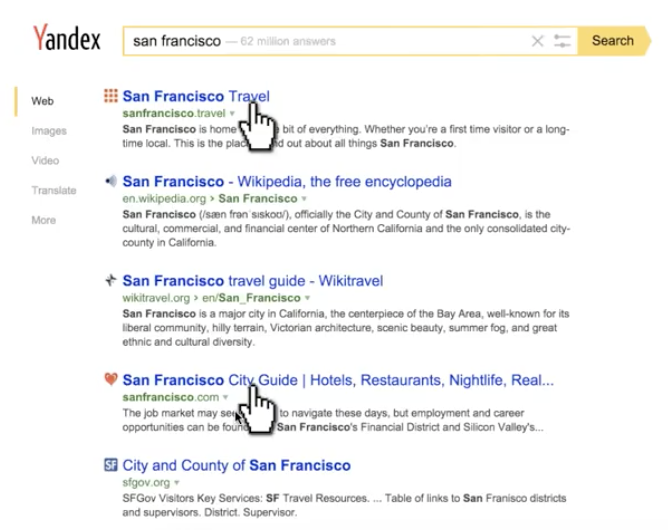
\includegraphics[scale=0.6]{figures/positionbased.png}
\end{figure}

Suppose we have the search results above and we observe the 2 clicks. How do we \textbf{model} this? \textbf{\textcolor{Maroon}{First}}, we randomly choose a result out of the 5, let's say we choose the 3rd one. We assume that the user first \textbf{\textcolor{Maroon}{examines}} the \textbf{snippet}. This is called the \textbf{\textcolor{Maroon}{probability of examination}}: $P_{exam}(3)$. This depends on the \textit{position}. \\
\\
\textbf{\textcolor{Maroon}{Secondly}}, if we like and think it is a good result for the \textbf{query}, we make another decision. Namely, we decide whether we are \textbf{\textcolor{Maroon}{attracted}} or not (by the snippet given our query). This is called \textbf{\textcolor{Maroon}{the probability of attractiveness}}: $P_{attr}(qd_3)$ (does not depend on examination). \\
\\
\textcolor{Maroon}{From lecture}: So see it as tossing 2 types of coins. First, you toss a coin from the \textbf{set of examination coins}, thereafter you toss a coin from the \textbf{set of attractive coins}. So you \textbf{\textcolor{Maroon}{click only}} if you \textbf{\textcolor{Maroon}{examine and find it attractive}}. Same applies for all 5 results $\{P_{exam}(1), P_{attr}(qd_1) \ldots P_{exam}(5), P_{attr}(qd_5)\}$.

\newpage

{\Large \textbf{Position-based model: \textcolor{MidnightBlue}{examination}}}:\\
{\large \textit{Terminology}}:
\begin{itemize}
    \setlength\itemsep{0em}
    \item \textbf{Examination} = reading a \textbf{\textcolor{Maroon}{snippet}}
    \item $E_r$ - binary random variable denoting examination of a snippet at rank $r$
\end{itemize}

{\large \textit{Position-based model (PBM)}}:
\begin{itemize}
    \setlength\itemsep{0em}
    \item Examination depends on rank: $P(E_r = 1) = \gamma_r$
\end{itemize}

So all \textcolor{Maroon}{probabilities of examination} will be replaced with $\gamma$, as following for example 5 results: $\{\gamma_1, P_{attr}(qd_1) \ldots \gamma_5, P_{attr}(qd_5)\}$. If the number of results is 100, then we would get 100 $\gamma$'s: $\{\gamma_1, \dots, \gamma_{100}\}$. \\
\\
\\
{\Large \textbf{Position-based model: \textcolor{MidnightBlue}{attractiveness}}}:\\
{\large \textit{Terminology}}:
\begin{itemize}
    \setlength\itemsep{0em}
    \item \textbf{Attractiveness} = a user wants to click on a document after examining it's \textbf{\textcolor{Maroon}{snippet}}
    \item $A_{qd}$ - binary random variable showing whethet document $d$ is attractive to a user, given query $q$
\end{itemize}

{\large \textit{Position-based model (PBM)}}:
\begin{itemize}
    \setlength\itemsep{0em}
    \item Attractive depends on a query-document pair: $P(A_{qd} = 1) = \alpha_{qd}$
\end{itemize} 

So all \textcolor{Maroon}{probabilities of attractiveness} will be replaced with $\alpha$, as following for example 5 documents: $\{\gamma_1, \alpha_{qd_1} \ldots \gamma_5, \alpha_{qd_5}\}$. If the number of documents is 100, then we would get 100 $\alpha$'s: $\{\alpha_{qd_1}, \dots, \alpha_{qd_{100}}\}$.\\
\\

\textbf{Position-based model: Summary}
\begin{itemize}
    \setlength\itemsep{0em}
    \item Probability of \textcolor{Maroon}{examination}: $P(E_{r_{d}} = 1) = \gamma_d$
    \item Probability of \textcolor{Maroon}{attractiveness}: $P(A_{qd} = 1) = \alpha_{qd}$
    \\
    \textcolor{red}{\rule{71ex}{1pt}}
    \item Probability of \textbf{\textcolor{Maroon}{click}}: $P(C_d = 1) = P(E_{r_{d}} = 1) \cdot P(A_{qd} = 1) = \gamma_d \cdot \alpha_{qd}$
\end{itemize}

\newpage
{\Large 1b). \textbf{Cascade model}: } 
\begin{enumerate}
    \setlength\itemsep{0em}
    \item Start from first document
    \item Examine documents one by one
    \item If click, then stop
    \item Otherwise, continue
\end{enumerate}

Again we \textcolor{Maroon}{click iff we examine and find it attractive}: $E_r = 1$ and $A_{d_{r}} = 1 \Leftrightarrow C_r = 1$.

The \textcolor{Maroon}{probability of attractiveness} stays the same, but there are some changes (see below): \\ 
\begin{minipage}{0.6\textwidth}
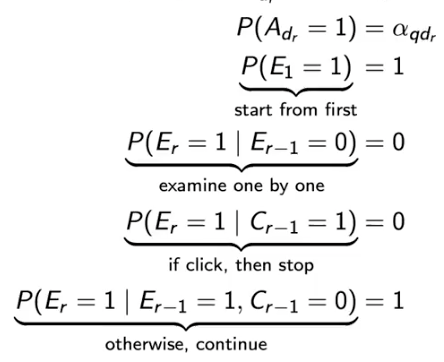
\includegraphics[scale=0.75]{figures/cascade.png}
\end{minipage}

\vspace{0.5cm}

{\Large \textbf{Basic click models summary}}: 
\begin{itemize}
    \setlength\itemsep{0em}
    \item Position-based model (PBM): \\
    + examination and attractiveness \\
    --  examination of a document at rank $r$ does not depend on examinations and clicks above $r$
    \item Cascade model (CM): \\
    + cascade dependency of examination at $r$ on examinations and clicks above $r$ \\
    -- only one click is allowed
\end{itemize}

\vspace{1cm}

{\huge 2). \textbf{Estimation} } \\
\\
\textbf{Parameter estimation}:
\begin{itemize}
    \setlength\itemsep{0em}
    \item Maximum likelihood estimation
    \item Expectation-maximization
    \begin{enumerate}
        \setlength\itemsep{0em}
        \item Set parameters to some initial values
        \item Repeat until convergence 
        \begin{itemize}
        \setlength\itemsep{0em}
            \item \textbf{E-step}: derive the expectation of the likelihood function
            \item \textbf{M-step}: maximize this expectation
        \end{itemize}
    \end{enumerate}
\end{itemize}

\vspace{0.5cm}

\textbf{EM update rules for PBM: \textcolor{Maroon}{attractiveness}} \\
\begin{minipage}{0.7\textwidth}
$ \alpha_{q d}^{(t+1)}=\frac{1}{\left|\mathcal{S}_{q d}\right|} \sum_{s \in \mathcal{S}_{q d}}\left(c_{d}^{(s)}+\left(1-c_{d}^{(s)}\right) \frac{\left(1-\gamma_{r}^{(t)}\right) \alpha_{q d}^{(t)}}{1-\gamma_{r}^{(t)} \alpha_{q d}^{(t)}}\right) $
\end{minipage}
\begin{minipage}{0.4\textwidth}
$t$: iteration \\
$S_{qd}$: search sessions iniated by query q and containing doc u \\
$c^{(s)}_d$: observed click on doc u in search sessions s
\end{minipage}

\vspace{0.5cm}

\textbf{EM update rules for PBM: \textcolor{Maroon}{examination}} \\
$ \gamma_{r}^{(t+1)}=\frac{1}{|\mathcal{S}|} \sum_{s \in \mathcal{S}}\left(c_{d}^{(s)}+\left(1-c_{d}^{(s)}\right)_{k} \frac{\gamma_{r}^{(t)}\left(1-\alpha_{q d}^{(t)}\right)}{1-\gamma_{r}^{(t)} \alpha_{q d}^{(t)}}\right) $

\vspace{0.5cm}

{\huge 3). \textbf{Applications} } \\
\\
\textbf{What can we get after estimation of a click model}?\\
\\
\begin{minipage}{0.5\textwidth}
\textcolor{Maroon}{Full probability} - probability that a user clicks on a document at rank $r$: $P(C_r = 1)$ \\
\\
\textcolor{Maroon}{Conditional probability} - probability that a user clicks on a document at rank r given previous clicks $P(C_r = 1 \mid C_1, \ldots, C_{r-1})$
\end{minipage}
\begin{minipage}{0.5\textwidth}
\;\;\;\; 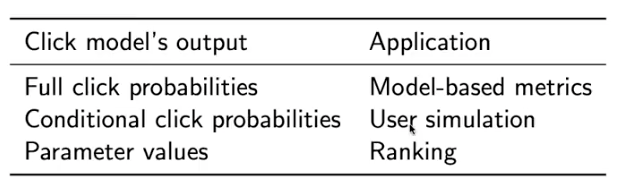
\includegraphics[scale=0.6]{figures/applications.png}
\end{minipage}

\vspace{0.65cm}

\textbf{Model-based metrics}: \\
\\
\begin{minipage}{0.5\textwidth}
Utitility-based metric: 
$$ \text { uMetric }=\sum_{r=1}^{n} P\left(C_{r}=1\right) \cdot U_{r}$$ 
Effort-based metric: 
$$\text { eMetric }=\sum_{r=1}^{n} P\left(S_{r}=1\right) \cdot F_{r}$$
\end{minipage}
\begin{minipage}{0.5\textwidth}
Expected reciprocal rank (ERR, second term last part from DBN): \\
\begin{align*}
    ERR &= \sum_r \frac{1}{r} \cdot P(S_r = 1) \\
    &= \sum_r \frac{1}{r} \cdot R_{qd_{r}} \cdot \prod^{r-1}_{i=1}(\gamma \cdot (1 - R_{qd_{i}})) 
\end{align*}
\end{minipage}

\vspace{0.25cm}
\begin{minipage}{0.5\textwidth}
Dynamic Bayesian network model (DBN) 
\begin{align*}
P\left(A_{r}=1\right) &=\alpha_{q d_{r}} \\
P\left(E_{1}=1\right) &=1 \\
P\left(E_{r}=1 \mid S_{r-1}=1\right) &=0 \\
P\left(E_{r}=1 \mid S_{r-1}=0\right) &=\gamma \\
P\left(S_{r}=1 \mid C_{r}=0\right) &=0 \\
P\left(S_{r}=1 \mid C_{r}=1\right) &=\sigma_{q d_{r}} \\
P\left(S_{r}=1\right) &=? 
\end{align*} 
\end{minipage}
\begin{minipage}{0.5\textwidth}
Dynamic Bayesian network model (DBN) 
\begin{align*}
P\left(S_{r}=1\right) &=P\left(S_{r}=1 \mid C_{r}=1\right) \cdot P\left(C_{r}=1\right) \\
&=\sigma_{q d_{r}} \cdot P\left(C_{r}=1\right) \\
&=\sigma_{q d_{r}} \cdot \alpha_{q d_{r}} \cdot P\left(E_{r}=1\right) \\
&=\sigma_{q d_{r}} \cdot \alpha_{q d_{r}} \cdot \prod_{i=1}^{r-1}\left(\gamma \cdot\left(1-\sigma_{q d_{i}} \cdot \alpha_{q d_{i}}\right)\right) \\
&=R_{q d_{r}} \cdot \prod_{i=1}^{r-1}\left(\gamma \cdot\left(1-R_{q d_{i}}\right)\right) \;\;(\textbf{ERR}).
\end{align*}
\end{minipage}

\newpage

\end{document}


%----------------------------------------------------------------------------------------

\end{document}
